\documentclass[11pt,a4paper,twoside,openright]{report}

\usepackage{graphicx}
\usepackage{tabularx}
\usepackage{subfigure}
\usepackage{afterpage}
\usepackage{amsmath,amssymb}            
\usepackage{rotating}  
\usepackage{fancyhdr}  
\usepackage[scriptsize]{caption} 
\usepackage{cite}
\usepackage{hyperref}
\usepackage{amsthm}
\usepackage{xargs}
\usepackage{cleveref}
\usepackage{algorithm}
\usepackage{algorithmicx}
\usepackage{algpseudocode}
\usepackage{units}
%\usepackage{wrapfig}
\usepackage{cutwin}
\usepackage[calc]{adjustbox}
% ===================================================
% PAGE LAYOUT
% ===================================================
\usepackage{geometry}    % Da rivedere
\geometry{
  inner=37.125mm,
  outer=33.4125mm,
  top=37.125mm,
  bottom=37.125mm,
  heightrounded,
  marginparwidth=51pt,
  marginparsep=17pt,
  headsep=24pt,
}
\setlength\parindent{0cm}
\setlength\parskip{1em}
\def\labelitemi{--}

%\linespread{1.1}

\usepackage[english]{babel}
\usepackage[utf8]{inputenc}
\renewcommand{\captionfont}{\normalfont \sffamily \itshape \small}



\pagestyle{empty}

% ===================================================
% THEOREMS
% ===================================================
\theoremstyle{plain}
\newtheorem{theorem}{Theorem}[chapter]
\newtheorem{lemma}[theorem]{Lemma}
\newtheorem{corollary}[theorem]{Corollary}

\theoremstyle{definition}
\newtheorem{definition}{Definition}[chapter]
\newtheorem{example}{Example}[chapter]

\theoremstyle{remark}
\newtheorem*{remark}{Remark}
\newtheorem*{note}{Note}


% ===================================================
% MACROS
% ===================================================
\newcommand{\smartdoubleflush}{\pagestyle{empty} \cleardoublepage \pagestyle{fancy}}


\newcommand{\EV}[2][]{{\mathbb{E}_{#1}\left[ #2 \right]}}

\newcommand{\vtheta}{{\boldsymbol{\theta}}}
\newcommand{\de}{\, \textrm{d}}
\newcommand{\sspace}{\mathcal{S}}
\newcommand{\aspace}{\mathcal{A}}
\newcommand{\tfunc}{\mathcal{P}}
\newcommand{\rfunc}{\mathcal{R}}
\newcommand*{\gradj}{\nabla_{\vtheta}J_\mu(\vtheta)}

\newcommandx{\poladv}[2][1, 2]{\mathbb{A}_{#1}^{#2}}
\newcommand{\norm}[2][1]{\left\| #2 \right\|_{#1}}
\newcommand{\transpose}[1]{{#1}^{\mathsf{T}}}
% ===================================================
% HEADERS AND FOOTERS
% ===================================================

\renewcommand{\chaptermark}[1]{\markboth{\chaptername\ \thechapter.\ #1}{}} 
\renewcommand{\sectionmark}[1]{\markright{\thesection.\ #1}}         
\fancyhead[LE,RO]{\bfseries\thepage}    
                                        
\fancyhead[RE]{\bfseries\leftmark}    
\fancyhead[LO]{\bfseries\rightmark}     
\renewcommand{\headrulewidth}{0.3pt}

\fancyfoot{} 

% ===================================================
% BEGIN DOCUMENT
% ===================================================

\begin{document}

\pagenumbering{roman}
\pagestyle{fancy}

\thispagestyle{empty}
%\begin{titlepage}
\vspace*{-1.5cm} \bfseries{
\begin{center}
  \LARGE
  POLITECNICO DI MILANO\\
  \vspace{0.2cm}
  
  \normalsize
  \textbf{{\Large S}CHOOL OF {\Large I}NDUSTRIAL AND {\Large I}NFORMATION {\Large E}NGINEERING} \\
  Master of Science in Computer Science and Engineering\\
  Department of Electronics, Information and Bioengineering\\
  \vspace{1cm}
  \begin{figure}[htbp]
    \begin{center}
      
\includegraphics[width=4.5cm]{pictures/newlogo}
%	
\psfig{file=./pictures/logopm.jpg,width=3.5cm}
    \end{center}
  \end{figure}
  \vspace*{0.3cm} \LARGE



  \textbf{Balancing Safety and Exploration in Policy Gradient}\\



  \vspace*{.75truecm} \large
  AI \& R Lab \\
  Artificial Intelligence \& Robotics Lab\\
   Politecnico di Milano
\end{center}
\vspace*{3.0cm} \large
\begin{flushleft}


  Supervisor: Prof. Marcello Restelli \\
  Co-supervisor: Dott. Matteo Papini 

\end{flushleft}
\vspace*{1.0cm}
\begin{flushright}


  Author:\\ Andrea Battistello, 873795\\ 


\end{flushright}
\vspace*{0.5cm}
\begin{center}



  Academic Year 2017-2018
\end{center} \clearpage
}

\smartdoubleflush
\vspace{17cm}

%\large
\begin{flushright}
\itshape{ A qualcuno...}
\end{flushright}

\smartdoubleflush

\normalfont

\chapter*{Abstract}
%\thispagestyle{empty}
\addcontentsline{toc}{chapter}{Abstract}

Safe Reinforcement Learning is necessary for critical applications, such as robotics, where exploratory behaviours can harm systems and people, but it also lends itself to economic interpretations. However, safe algorithms often tend to be overly conservative, sacrificing too much in terms of speed and exploration. The latter, in particular, is of fundamental importance for a learning algorithm to gain informations about the environment. In this thesis, we will investigate the non-trivial tradeoff between these two competing aspects, safety and exploration. 
Starting from the idea that a practical algorithm should be safe as needed, but no more, we identify interesting application scenarios and propose Safely-Exploring Policy Gradient (SEPG), a very general policy gadient framework that can be customized to match particular safety constraints. To do so, we generalize existing bounds on performance improvement for Gaussian policies to the adaptive-variance case and propose policy updates that are both safe and exploratory. 

\smartdoubleflush

\chapter*{Estratto in lingua italiana}
%\thispagestyle{empty}
\addcontentsline{toc}{chapter}{Estratto in lingua italiana}

Ogni giorno dobbiamo compiere delle scelte: scegliamo quali vestiti indossare, se è più conveniente prendere l'autobus o la metropolitana, se impostare la sveglia per il giorno successivo e così via. Noi abbiamo imparato come affrontare questi problemi da quando eravamo bambini. Il processo che ci ha portato ad acquisire questa capacità è lungo e complesso, ma può essere suddiviso in pochi elementi essenziali: i) abbiamo una percezione di ciò che ci circonda, ii) possiamo interagire con l'ambiente compiendo delle azioni e iii) l'ambiente reagisce dandoci una nuova percezione. Questi tre fattori entrano sempre in gioco quando vogliamo apprendere una nuova abilità (\eg giocare a tennis). 
Questa interazione con ciò che ci circonda costituisce ciò che chiamiamo esperienza. Tuttavia, l'esperienza da sola non è sufficiente: dobbiamo anche identificare un obiettivo. In termini molto semplici, possiamo dire che siamo felici se l'obiettivo è stato raggiunto, altrimenti siamo tristi. La quantità di felicità (o tristezza) che otteniamo può essere vista come una ricompensa che l'ambiente ci offre. Ciò che istintivamente impariamo a fare è sviluppare delle strategie che aumentino la quantità di felicità ottenuta tramite la nostra interazione con l'ambiente. Un esempio molto calzante è dato dal processo di addestramento dei cani: il cane impara a stare seduto perché sa che poi riceverà una ricompensa.\\
Questo processo di apprendimento, quando applicato a programmi informatici, prende il nome di apprendimento per rinforzo.



L'apprendimento per rinforzo (RL) è un campo dell'intelligenza artificiale che imita il modo in cui gli esseri viventi apprendono in natura. Questi algoritmi di apprendimento si basano su un modello matematico semplificato ma potente che è in grado di descrivere le interazioni tra un agente e l'ambiente.
%
%In questo lavoro esploreremo l'approccio computazionale all'apprendimento per rinforzo, considerando un modello matematico semplificato ma potente.
Il risultato finale sarà una funzione che associa, per ogni possible situazione, l'azione che l'agente deve compiere per massimizzare la ricompensa che potrà ricevere.


Queste ricompense hanno lo scopo di fornire informazioni su \textit{cosa} è l'obiettivo da perseguire ma non su \textit{come} fare per raggiungerlo. All'agente non viene detto quali azioni intraprendere, piuttosto, deve scoprire da solo quali azioni sono le più redditizie. 
L'agente può imparare il valore delle proprie azioni procedendo per tentativi e accumulando esperienza.\\
Questo non è un compito banale, dal momento che le azioni possono potenzialmente avere effetti a lungo termine. Infatti, un'azione influisce sullo stato successivo, da cui un'altra azione può condurre a un altro stato ancora e così via, generando una sequenza di eventi causalmente correlati. Le ricompense a lungo termine e la ricerca per tentativi sono i due aspetti più importanti dell'apprendimento per rinforzo, che rendono questo problema difficile ma intrigante.

Tra le sfide attuali nell'ambito dell'apprendimento per rinforzo, compare il problema di come esplorare l'ambiente e di come farlo in modo sicuro. L'esplorazione è un aspetto fondamentale dell'apprendimento, poiché risolvere efficacemente un compito difficile richiede anche creatività. In questo contesto, l'esplorazione è intesa come prendere azioni che sono diverse da quelle a cui l'agente è abituato. Cambiare leggermente il modo in cui facciamo qualcosa può aiutarci ad acquisire una maggiore conoscenza dell'ambiente e potenzialmente può aiutarci a trovare nuove soluzioni. Tuttavia, un eccesso di esplorazione non è sempre utile e può danneggiare macchine e persone, oltre ad avere un possibile impatto economico. Ad esempio, possiamo pensare a un braccio robotico che sta imparando a colpire una palla con una mazza da baseball. Può accadere che, durante la fase di apprendimento, il braccio robotico agiti la mazza con un movimento brusco, il quale potrebbe potenzialmente rompere il macchinario. Questo problema si riflette economicamente anche nei costi di riparazione del braccio robotico.

In questa tesi vogliamo combinare questi due aspetti contrastanti di sicurezza durante l'apprendimento ed esplorazione, ed escogitare una soluzione generale che possa essere adattata alle esigenze dell'utente. Ci concentreremo su una particolare classe di algoritmi di apprendimento, chiamata 'policy gradient'~\cite{peters}. Oltre ad avere buone proprietà di convergenza, questi metodi sono particolarmente adatti per i problemi di controllo con azioni continue, in quanto sono in grado di risolvere molte delle difficoltà che si presentano in questo campo, come lo spazio di stati multidimensionale e sensori non precisi. Inoltre, consentono di integrare facilmente delle conoscenze specifiche sul dominio del problema al fine di progettare soluzioni più sicure e più efficaci. Il lavoro fatto recentemente nel campo dell'apprendimento per rinforzo sicuro, ha portato a buoni risultati teorici. In particolare faremo riferimento al lavoro di Kakade e Langford~\cite{Kakade02approximatelyoptimal} su 'conservative policy iteration', successivamente perfezionato da Pirotta et al. \cite{safe_iteration} e adattato al metodo policy gradient in ~\cite{adaptive_step}. Tuttavia, questi risultati non considerano il fattore esplorativo, che è di grande importanza nell'apprendimento. Inoltre, i risultati presentati in questo campo, fanno riferimento principalmente al caso limitato di miglioramenti monotoni, in cui l'obiettivo principale è migliorare la soluzione corrente ad ogni iterazione. Questo vincolo, tuttavia, ha un forte impatto sulla velocità di apprendimento, dal momento che dobbiamo fare aggiornamenti molto piccoli per migliorare in modo sicuro la soluzione corrente. Per questo motivo, i metodi introdotti precedentemente sono noti per essere eccessivamente cauti, in quanto sacrificano troppo in termini di velocità di apprendimento ed esplorazione.

Partendo da questi risultati, introdurremo un nuovo framework per l'apprendimento per rinforzo sicuro. Questo framework va oltre il singolo caso di miglioramento monotono, e includerà diversi tipi di vincoli, ciascuno corrispondente a una diversa esigenza pratica. L'utente, quindi, potrà scegliere il vincolo di sicurezza che meglio si adatta alle sue esigenze, senza garantire più di quanto sia necessario. All'interno di questo framework, estenderemo i risultati di Pirotta et al.~\cite{adaptive_step} per occuparci anche dell'esplorazione adattiva. Il contributo finale che presenteremo in questo lavoro è un algoritmo generale denominato Safely-Exploring Policy Gradient (SEPG), che combina i nuovi risultati sviluppati in questa tesi. SEPG può essere personalizzato per soddisfare i diversi vincoli di sicurezza descritti nel nuovo framework appena introdotto.
\smartdoubleflush
\chapter*{Ringraziamenti}
\thispagestyle{empty}
\addcontentsline{toc}{chapter}{Ringraziamenti}

\smartdoubleflush

 


\tableofcontents 
\smartdoubleflush


\chapter{Introduction}
\label{ch:intro}
%\thispagestyle{empty}
\pagenumbering{arabic}
\setcounter{page}{1}


Every day we are required to make some choices:  we choose what to wear everyday, if it is more convenient to take the bus than the metro, whether to put the alarm for the next day and so on. We, as decision-makers, have learned how to tackle these problems since we were children. The process that brought us to acquire this ability is long and complex, but it can be broken down to few essential pieces: i) we have a perception of what is surrounding us, ii) we can interact with the environment by taking some actions and iii) the environment reacts by giving us a new perception. These three factors always come into play, whether we want to learn a new skill (\eg to play the piano), we want to play a game and so on. This interaction with the environment builds what we call experience. However, experience alone is not enough: we also have to identify a goal. In a very simple setting, we can say that we are happy if the accomplish the goal, otherwise we are sad. The amount of happiness (or sadness) can be seen as a reward that the environment gives us. What we naturally learn to do is to develop strategies that increase the amount of happiness obtained by our interaction with the environment. This process of learning, when applied to computer programs, takes the name of reinforcement learning.



Reinforcement Learning (RL) is a field of Machine Learning that closely resembles how living beings learn in nature. RL algorithms are based on a simplified yet powerful mathematical model that is able to describe the interactions between an agent and the environment.
%
%In this work we will explore the computational approach to learning from interaction, by considering a simplified yet powerful mathematical model. 
The final result will be a function that maps states to actions, that tells the agent what to do, so as to maximize the reward that it is able to gain. This reward signal is intended to give insights about \textit{what} is the goal to pursue but not \textit{how}. The learner is not told which actions to take, but rather it has to discover which actions are more valuable via trial-and-error, from experience. \\
This is not a trivial task, since actions can potentially have long-term effects. As a matter of facts, an action affects the following state, from where another action can lead to another state and so on, generating a sequence of causally related events. Delayed rewards and trial-and-error search are the two most important aspects of reinforcement learning, that make this problem both difficult and intriguing.

Among the current challenges that reinforcement learning has to take, there are the inner difficulties of exploring the environment and how to do it safely. Exploration is a fundamental aspect of learning, as it requires creativity and practice to effectively solve a difficult task. In this context, exploration is intended as taking actions that are different than the ones we are used to take. Slightly changing the way we do something can help you gain more knowledge about the environment, and potentially can help find new solutions. However, an excess in exploration is not always useful and can harm systems and people, besides having an intuitive economical impact. As an example, we can think of a robotic arm that is learning how to hit a ball with a baseball bat. It can happen that, during the learning phase, the robotic arm swings the bat with sudden movements, that could potentially break the system. This problem is also reflected in the costs of repairing the robotic arm.

In this thesis, we want to combine the two competing aspects of safety and exploration, and devise a general solution that can be customized to the user needs. We will focus on a particular class of algorithms in the reinforcement learning literature called policy gradient methods~\cite{peters}. Besides having nice convergence properties, these methods are particularly suited for control tasks with continuous actions, as they are able to address many of the difficulties that arise in this field, such as high dimensional state spaces and noisy sensors. Moreover, they allow to easily incorporate prior domain knowledge in order to design safer and more effective results. Recent works in safe reinforcement learning have brought to nice theoretical results, but do not consider the exploration factor. In particular, we will refer to the work of Kakade and Langford~\cite{Kakade02approximatelyoptimal} on conservative policy iteration, later refined by Pirotta et al.~\cite{safe_iteration} and adapted to the policy gradient method in~\cite{adaptive_step}. Moreover, the results presented in this field mostly consider the restricted case of monotonic improvements, where the main goal is to improve the current solution at every iteration. This constraint, though, has a big impact on the learning speed of the algorithm, since we need to take very small updates to safely improve the current solution. For this reason, these methods are known to be overly conservative, as they sacrifice too much in terms of speed and exploration. 

Starting from these results, we will introduce a new framework for safe reinforcement learning. This framework goes beyond the single monotonic improvement case, and it will include several kind of constraints, each corresponding to a different practical needs. The user can then choose the type of safety constraint that better suits his requirements, without guaranteeing more that what is needed. Within this framework, we will extend the results from~\cite{adaptive_step} to also deal with adaptive exploration. The final contribution that we introduce in this work is a general algorithm named Safely-Exploring Policy Gradient (SEPG), that combines the new results developed in this thesis. SEPG can be customized to match several safety constraints described in the newly adopted framework. 

The contents of the thesis are organized as follows. In \Cref{ch:rl} we will provide an overview of reinforcement learning and we will introduce the basic concepts that are needed to define policy gradient methods. In particular we will define a mathematical model called Markov Decision Process that describes the interactions between the agent and the environment. In \Cref{ch:safepg} we will describe in details the main results on safe reinforcement learning. Specifically, we will start from the results of Kakade and Langford~\cite{Kakade02approximatelyoptimal} on conservative policy iteration, that were later extended by~\cite{safe_iteration} with the introduction of a tighter bound on performance improvement. Pirotta et al.~\cite{adaptive_step} adapted these results to policy gradient, that were later extended by Papini et al.~\cite{adaptive_batch} to also include the batch size. In \Cref{ch:balance} we will introduce the main contribution of this thesis. We will first provide the new safe reinforcement learning framework where we identify two main classes of safety  constraints. Then, we will derive new results for the adaptive exploration case and finally we will see how to include these results in a practical algorithm (SEPG). We will describe in details how to adapt SEPG to match every safety constraint. Next, in \Cref{ch:experim} we will evaluate SEPG variants on simulated continuous control tasks. We will also compare SEPG with other non-safe approaches and we will analyse the results. Finally, in \Cref{ch:conclusion} we will derive some conclusions and we will describe possible additions that can be studied in future works.
 



%Reinforcement Learning is a field of machine learning that closely resembles how living entities learn in nature. We are able to learn by observing how the environment reacts to our actions. With a careful model designed to describe this interaction, we are able to apply this concept computationally. 
%
%The idea that we learn by interacting with our environment is probably the first to occur to us when we think about the nature of learning. When an infant plays, waves its arms, or looks about, it has no explicit teacher, but it does have a direct connection to its environment. Exercising this connection produces a wealth of information about cause and effect, about the consequences of actions, and about what to do in order to achieve goals. Throughout our lives, such interactions are undoubtedly a major source
%of knowledge about our environment and ourselves. Whether we are learning to drive a car or to hold a conversation, we are acutely aware of how our environment responds to what we do, and we seek to influence what happens through our behavior. Learning from interaction is a foundational idea underlying nearly all theories of learning and intelligence.

 \smartdoubleflush
\chapter{Reinforcement Learning}
\label{ch:rl}
%\thispagestyle{empty}

In this chapter, we will formalize the problem of reinforcement learning using a model taken from dynamical systems theory called Markov decision process. This model is able to capture the main aspects that build an interaction between the agent and the environment: observations, actions and goal. This model will be described in details in \Cref{sec:mdp}. Next, three general methods to solve a MDP are presented in \Cref{sec:solve-mdp}: policy iteration, value iteration and policy search. We will briefly describe the former two methods, enough to introduce a policy search method called Policy Gradient, that is the main interest of this work. Policy Gradient methods will then be described in detail in \Cref{sec:policy-gradient}, including some aspects about gradient approximation, baselines and other more advanced refinements.








\section{Markov Decision Processes}
\label{sec:mdp}
In this section we will give a formal definition of reinforcement learning by defining a mathematical model called Markov decision process. For a complete treatment of reinforcement learning, refer to \cite{sutton1998reinforcement}.\\
The main aspects that we want to capture are the interactions between an agent and the environment over time. A learning agent must be able to sense the state of its environment and take some actions, while the environment itself receives the actions from the agent and reacts by changing the state and giving feedbacks to the agent,completing a cycle.
The agent must also have a goal that is related to a state of the environment.\\
Markov decision processes are intended to include just these three aspects -- sensation, action and goal -- in their simplest possible forms without trivializing any of them.
\newpage
\begin{definition}
A Markov Decision Process (MDP) is a tuple $\left\langle \sspace, \aspace, \tfunc, \rfunc, \gamma, \mu \right\rangle$  where:
\begin{itemize}
\item $\sspace$ is the set of possible \textbf{states}
\item $\aspace$ is the set of possible \textbf{actions}
\item $\tfunc : \sspace \times \aspace \rightarrow \Delta (\sspace)$ is the \textbf{transition function} that, given the current state and current action, outputs a probability distribution over the next state.
\item $\rfunc : \sspace \times \aspace \rightarrow \mathbb{R}$ is the \textbf{reward function} that maps a scalar reward to every state-action pair
\item $\gamma$ is the \textbf{discount factor}
\item $\mu : \Delta ( \sspace )$ is a probability distribution over the \textbf{initial state}. 
\end{itemize}
\end{definition}

%At each time step $t$, the agent receives observations from the environment. From the current observations and previous interactions, the agent builds a representation of the current state of the environment, $s_t$ . Then, depending on $s_t$, it takes action $a_t$. Finally, it is given a (possibly negative) reward depending on how much its behaviour is compliant with the goal, in the form of a scalar signal $r_{t+1}$. 
The dynamics of the environment, as represented by the agent, must satisfy two fundamental properties:
\begin{itemize}
\item[-] Stationarity: the transition function $\tfunc$ does not change over time.
\item[-] Markov property: the transition function $\tfunc$ only depends on the previous state, not on the entire history of the interaction.
\end{itemize}

An agent in a MDP starts from an initial state drawn from the probability distribution $\mu$, $s_0 \sim \mu$. From this state, the agent can interact with the environment by executing an action $a_0 \in \aspace$. The environment receives action $a_0$ and reacts to this stimulus by returning to the agent the next state $s_1$ drawn from the transition function $s_1 \sim \tfunc(s_0, a_0)$ and a scalar reward $r_1 = \rfunc(s_0, a_0)$. From its new observation, the agent can continue the interaction with the environment by choosing another action $a_1$ and so on until it reaches the goal. We define the  sequence of collected states, actions and rewards $\tau \sim s_0, a_0, s_1, r_1, a_1, s_2, \ldots$ as a trajectory. Sometimes we will refer to a trajectory with terms like 'sample' or 'experience', since the collected information will be used for the learning procedure.

\Cref{fig:mdp-example} shows a graphical representation of a MDP. The circles represent the states of the environment and the arrows represent the transition probability of going from $s_t$ to $s_{t+1}$. Each state is associated with a reward, depicted in red. \\
Assuming that a student starts from Class 1, he can be distracted and use the phone to access Facebook with probability $0.5$. If this happens, the environment will transition to the new state and the student will receive a reward of $-1$. From this new state it would be hard for the student to return to Class 1, because there is a $0.9$ probability of continuing to use Facebook (and receiving a negative reward). The goal, in this simple example, is to go to sleep.\\
This mathematical model is very general and can be used also to model more complex problems. 

\begin{figure}[t]
\centering
\includegraphics[width=0.9\textwidth]{pictures/mdp_agent_environment}
\caption{Agent-environment loop}
\end{figure}

\begin{example}[Chess]
The game of chess can be modelled as an MDP with a discrete state space that encodes the position of all the pieces in the checkerboard, a discrete action space encoding all the possible moves of the pieces, a deterministic transition function that follows the rules of the game and a (possible) reward function:
\begin{equation*}
\rfunc(s,a) = \begin{cases}\,\,\,\,\,1 & \textrm{Player wins} \\ -1 & \textrm{Player does not win} \end{cases}
\end{equation*}
\end{example}


\renewcommand\windowpagestuff{\centering 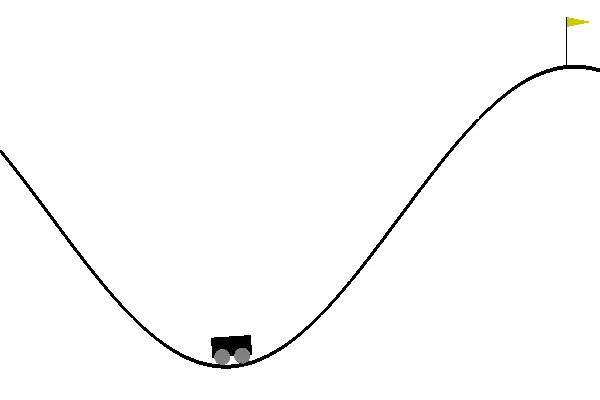
\includegraphics[width=5.5cm]{pictures/mountain_car} \captionof{figure}{Mountain car task}}
\opencutright

\begin{adjustbox}{valign=C,vspace=0bp,minipage={1.0\linewidth}}
\begin{example}[Mountain Car]\label{example:mc}
\begin{cutout}{0}{7.5cm}{0pt}{12}
A car is placed between two hills and can move left or right. The goal is to reach the top of the right hill, but the engine is not powerful enough to directly climb the hill, so the optimal solution is to gain momentum by first going in the opposite direction. This task can be modelled with a continuous state space $\sspace \in [-2, 2]$, a continuous action representing the force applied to the car, $\aspace \in [-1, 1]$, a deterministic transition function given by the laws of physics and the following reward function:
\end{cutout}

\begin{equation*}
\rfunc(s,a) = \begin{cases} +100 & \textrm{when } s \geq 1.5 \\ -a^2 & \textrm{otherwise} \end{cases}
\end{equation*}

This problem is particularly difficult for its exploration need: the agent is not aware of the presence of the goal until it is reached. Therefore, the agent needs to take actions that possibly have a bad impact on the immediate reward in order to reach the goal and being able to solve the problem. This concept of exploration (take actions to gain informations about the environment) vs exploitation (take actions that you know are profitable) will be described in the next chapter.
\end{example}

\end{adjustbox}


\renewcommand\windowpagestuff{\centering 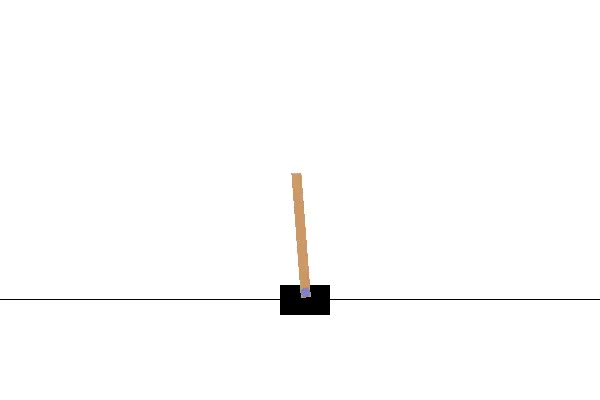
\includegraphics[width=5.5cm]{pictures/cartpole} \captionof{figure}{Cartpole task}}
\opencutleft
\begin{adjustbox}{valign=C,vspace=0bp,minipage={1.0\linewidth}}
\begin{example}[Cartpole]

\begin{cutout}{3}{0pt}{8cm}{13}
A pole is attached to a cart by a joint that is free to rotate. The cart moves along a frictionless track either left or right. The pole starts upright (with a small perturbation), and the goal is to prevent it from falling over by moving the cart left or right.\\
This task can be modelled with a continuous multidimensional state space $\sspace \in \mathbb{R}^4$. The state features are: the position of the cart $s_0 \in [-2.4, 2.4]$, its velocity $s_1 \in [-\infty, \infty]$, the pole angle $s_2 \in [-\frac{\pi}{2}, \frac{\pi}{2}]$ and its angular velocity $s_3 \in [-\infty, \infty]$. The action space is continuous $\aspace \in [-1, 1]$ and represents the force to be applied on the cart. The transition function is given by the laws of physics and the reward is $+1$ for every step until the episode ends. An episode ends when a maximum step limit $H$ is reached or when the pole is inclined more than 15 degrees from the vertical.


\end{cutout}

\end{example}
\end{adjustbox}


%An agent in a MDP starts from an initial state drawn from the probability distribution $\mu$, $s_0 \sim \mu$. From this state, the agent can interact with the environment by executing an action $a_0 \in \aspace$. The environment receives action $a_0$ and reacts to this stimulus by returning to the agent the next state $s_1$ drawn from the transition function $s_1 \sim \tfunc(s_0, a_0)$ and a scalar reward $r_1 = \rfunc(s_0, a_0)$. From its new observation, the agent can continue the interaction with the environment by choosing another action $a_1$ and so on until it reaches the goal. We define the  sequence of collected states, actions and rewards $\tau \sim s_0, a_0, s_1, r_1, a_1, s_2, \ldots$ as a trajectory. Sometimes we will refer to a trajectory with terms like 'sample' or 'experience', since the collected information will be used for the learning procedure.



Intuitively, the agent aims at maximizing the sum of the collected rewards. However, this na\`ive sum of rewards do not apply if we consider infinite-horizon MDPs, which is a common setting in the literature. In fact, summing over potentially infinite-length trajectories will cause the cumulative reward to grow indefinitely and lose its original meaning. (e.g. earning +1 at every step will have the same meaning of earning +100 at every step, since over an infinite horizon they will both grow to infinity).\\
For this reason, it is common to consider a generalized version where we apply a discount factor $\gamma$ to the immediate reward and consider the cumulative discounted reward:
\begin{definition}[Cumulative discounted reward]
\begin{equation*}
R(\tau) = \sum_{t=0}^{\infty} \gamma^t r_t
\end{equation*}
where $\gamma \in [0,1]$ is called discount factor. 
\end{definition}
Note that the naive cumulative reward can be obtained by setting $\gamma=1$, and this is sometimes used when the horizon is finite. 

\begin{figure}[t]
\centering
\begin{subfigure}[t]{0.495\textwidth}
\includegraphics[width=\textwidth]{pictures/mdp_example}
\caption{Visual representation of the transition function (black) and reward function (red)}
\end{subfigure}
\hfill
\begin{subfigure}[t]{0.495\textwidth}
\includegraphics[width=\textwidth]{pictures/mdp_policy}
\caption{Visual representation of a (deterministic) policy}
\end{subfigure}
\caption{Representation of a simple MDP} \label{fig:mdp-example}
\end{figure}

However, the addition of the discount factor has a well-known two-fold meaning: at a first glance, it represents how the agent is interested in future rewards. With $\gamma$ close to $0$, we have a myopic behaviour, where we are only interested in immediate rewards rather than long-term investments. With $\gamma$ close to $1$, instead, we are giving more value to long-term rewards. In the second place, $\gamma$ can also represent the probability that the simulation will continue for one more step. If $\gamma$ is low, we should strive to get as much as we can because we don't have any assurance that we could last one more step.
The discount factor usually depends on the domain and the goal that we want to achieve: a long-term goal will require a value of $\gamma \simeq 1$.


The actual value of the discounted cumulative reward depends on the interaction of the agent with the environment over a trajectory. Many factors come into play to influence this objective function, most importantly the behaviour of the agent (i.e., which actions the agent chooses). The way an agent interacts with the environment, hence its behaviour, is defined by the policy function:
\begin{definition}
A policy $\pi: \sspace \rightarrow \Delta (\aspace)$ is a function that for each state $s \in \sspace$, outputs a probability distribution over the actions in $\aspace$. In other words, from state $s$ the agent will choose action $a$ with probability $\pi(a \mid s)$.
\end{definition}

The policy is one of the main ingredients of reinforcement learning, as it is the final result of a reinforcement learning algorithm. The policy tells the agent which actions to choose in every state.
Starting from an initial state $s_0$, the agent will choose action $a_0 \sim \pi(\cdot | s_0)$ drawn from the action distribution induced by the policy in this state. \\
Given an initial state and a policy, we can define its performance, or expected return, in this way:
\begin{definition}[Performance of a policy $\pi$]
The performance (or expected return) of a policy $\pi$ under initial state distribution $\mu$ is:
\[
J_\mu(\pi) = \EV[{\genfrac{}{}{0pt}{}{a_k \sim \pi, s_0 \sim \mu}{s_k \sim \tfunc \hspace{20pt}}}]{R},
\]
that is, the expected value of the discounted cumulative reward obtained by following the policy $\pi$ starting from an initial state drawn from $\mu$.
\end{definition}
Having defined this new metric, we can easily rank each policy according to its performance: a policy $\pi_1$ is better than a policy $\pi_0$ if $J_\mu(\pi_1) > J_\mu(\pi_0)$. The next step will be to find the policy that achieves the highest performance for a given MDP. This is the goal of solving an MDP.

\textbf{Problem formulation:}\quad
To solve a MDP means to find an optimal policy $\pi^*$ that maximizes the average cumulative reward. More formally we want to find $\pi^*$ such that $J_\mu(\pi^*)=\EV[a_k \sim \pi^*, s_0 \sim \mu]{R}$ is maximum.

Summing up, we can define the interaction between an agent and the environment as a sequence of state-action-reward tuples called a trajectory. The environment is modelled with a markovian transition function - a function that takes the current state-action pair and outputs a probability distribution over the next state. The Markov property assures that the transition function depends only on the current state and not on the entire history of interactions. The agent receives a reward for every action it takes and aims at maximizing the discounted cumulative reward. The behaviour of the agent is characterized by the policy function $\pi$, which yields, for every state $s$, a probability distribution over actions $\pi(a|s)$. Every policy can be ranked by its performance or expected reward, obtained following the policy from an initial state drawn from $\mu$. A MDP is considered solved when we find an optimal policy $\pi^*$ whose performance value is maximal. For every stationary MDP, there exists an optimal policy that is deterministic, namely, a policy that for each state yield a single action with probability 1.

Here we define a new quantity that will be useful later which is the discounted future state distribution. This function calculates the visitation frequency for each state $s\in\sspace$ by starting from $s_0\sim\mu$ and following policy $\pi$. This quantity is defined as follows:
\begin{definition}[Future state distribution]
The (discounted) future state distribution is defined as: 
\[
d_{\mu}^{\pi}(s) = (1-\gamma)\sum_{t=0}^{\infty} \gamma^t Pr(s_t = s)
\]
This quantity identifies the expected state distribution starting from $s_0 \sim \mu$ and following policy $\pi$. 
\end{definition}

Following this definition, we can reformulate the performance of a policy $\pi$ as a function of the state distribution $d_\mu^\pi(s)$.

\begin{definition}[Performance given state distribution]
The performance of a policy $\pi$ given an initial state distribution $\mu$ can be expressed as: 
\begin{equation*}
J_{\mu}(\pi) = \int_{\sspace} d_{\mu}^{\pi}(s) \int_{\aspace} \pi(a \mid s) \rfunc(s,a) \de a \de s
\end{equation*}
\end{definition}


\subsection{Value functions}
So far we have defined what is a MDP and what it means to find an optimal policy $\pi^*$. In this section, we will take the problem under a different perspective by considering the value of each state. The value of a state should consider not only immediate rewards, but also the discounted sum of all the rewards that the agent may get. This idea of including delayed rewards to describe the value of a state is implemented by the state-value function:

\begin{definition}[State-value function]
The value of a state $s$ that can be obtained by running policy $\pi$ is given by:
\[
V^{\pi}(s) = \int_{\aspace} \pi(a \mid s) \left( \rfunc(s,a) + \gamma \int_{\sspace} \tfunc(s' \mid s, a) V^{\pi} (s') \de s' \right) \de a.
\]
\end{definition}

The state-value function $V^\pi(s)$ encodes the average reward that we will obtain starting from state $s$ and following $\pi$ thereafter. Note that this is a recursive definition, as to compute the value of state $s$ we need to compute the values of all the states reachable from $s$ and so on. This definition allows us to give a different way to calculate the performance of a policy based on the value function and the initial state distribution:
\[
J_\mu(\pi) = \int_{\sspace}\mu(s)V^\pi(s)\de s.
\]
The value of the optimal policy $\pi^*$ is called optimal state-value function $V^*(s) = V^{\pi^*}(s)$. The optimal value function is unique, even if multiple optimal policies may exist\footnote{A MDP can have multiple optimal policies, but what we are mainly concerned about is that at least one of them is deterministic and has the same value function of other optimal stochastic policies.}. We can restate the goal of an RL algorithm as a maximization over the policy space of the state-value function for all states:
\[
\pi^* = \arg\max_{\pi \in \Pi} V^\pi(s),\qquad \forall s \in \sspace.
\]
The value function is useful evaluate policies, however it does not say anything about the actions that brought to that value. Since our main goal is to find an optimal policy, we need a way to assign a value also to the actions. The following statement will define the action-value function:

\begin{definition}[Action-value function]
The action-value function for a policy $\pi$ is defined as follows:
\[
Q^{\pi}(s, a) = \rfunc(s, a) + \gamma \int_{\sspace} \tfunc (s' \mid s, a) \int_{\aspace} \pi(a' \mid s') Q^{\pi} (s', a') \de a' \de s'
\]
\end{definition}

The action-value function defines the value that we can obtain starting from state $s$, executing action $a$ and following policy $\pi$ thereafter. This function encodes more information, since we can retrieve the state-value function by averaging the action-value function over all actions: $V^\pi(s) = \EV[a\in\aspace]{Q^\pi(s,a)}$. \\
Similarly to the definition of the optimal value function, the optimal action-value function $Q^*$ is defined to be the action-value function of the optimal policy: $Q^*(s) = Q^{\pi^*}$. 

The action-value function let us introduce another quantity of particular interest for the algorithms described in \Cref{sec:solve-mdp}, called the advantage function. The advantage of action $a$ over policy $\pi$ encodes how much we can gain by performing action $a$ instead of following the policy $\pi$, and is defined as follows:
\begin{definition}[Advantage function]
The advantage function of action $a$ over policy $\pi$ in state $s$, is defined as:
\[
A^{\pi}(s,a) = Q^{\pi}(s,a) - V^{\pi}(s)
\]
\end{definition}

The advantage function can also be used to compare two policies $\pi'$ and $\pi$: for every state $s$ we compute the advantage of selecting an action from $\pi'$ rather than $\pi$. In this case, it is called policy advantage function.
\begin{definition}[Policy advantage function]
The advantage of policy $\pi'$ with respect to policy $\pi$ in state $s$ can be computed as:
\[
A_\pi^{\pi'}(s) = \int_{\aspace} \pi'(a|s)A^\pi(s, a) \de a,
\]
whose expected value over the states is called expected policy advantage function:
\[
\poladv[\pi,\mu][\pi'] = \int_{\sspace} d_\mu^{\pi}(s)A_\pi^{\pi'}(s) \de s.
\]
\end{definition}


\section{General methods to solve a MDP}
\label{sec:solve-mdp}

In the previous section we have seen that solving a MDP means finding the optimal policy $\pi^*$ with the highest performance $J_\mu(\pi)$, which yields the optimal state-value function $V^*(s)$. Before diving into specific methods that aim at solving a MDP, we will provide some classification for learning algorithms.\\
First of all, we have to distinguish between a \textit{target} policy and a \textit{behaviour} policy: the target policy is the output of the algorithm, the one that is intended to solve the MDP. The behaviour policy, instead, is a policy that is used to collect the trajectory samples that will be used for learning. Depending on how the trajectories used to learn the target policy are collected, a learning algorithm can operate on-policy or off-policy:
\begin{itemize}
\item \textbf{On-policy}: the behaviour policy corresponds to the target policy. This means that every collected trajectory is sampled from the current policy. In simpler terms, it means that the agent learns from its own experience.
\item \textbf{Off-policy}: the target policy differs from the behaviour policy. In this case, the agent will learn from 'someone else'. Note that 'someone else' can also mean from itself in a different time-frame.
\end{itemize}

Another difference between the learning algorithms arises when we consider the degree of knowledge about the environment that the agent has:
\begin{itemize}
\item \textbf{Model-based}: the agent has a model of the environment, which can be either exact or approximated. Note that if the agent has an exact model, then the MDP can be solved even without experience.
\item \textbf{Model-free}: the agent has no information about the environment. The only way to learn is by collecting samples from the environment.
\end{itemize}

This concludes our partial taxonomy of RL methods. Of course, there are other aspects that are used to classify a RL method, but these are out of scope for this work. We will only consider model-free on-policy methods. This is a common scenario for  control problems where it is possible to collect samples from the environment, but it may not be possible to build an exact model of it.\\
The following sections will describe the three main approaches that are used to solve a MDP: policy iteration, value iteration and policy search.

\subsection{Policy iteration}
As we have seen in the previous section, the state-value function associates a value to each state of a MDP by considering all the discounted future rewards that can be taken by following a policy $\pi$ from that state. The state-value functions associated to different policies can be used to define an ordering relationship between policies:

\begin{definition}[Policy improvement]
Given two policies $\pi, \pi'$, policy $\pi'$ is better than or equal to ($\succcurlyeq$) policy $\pi$ when the value function of $\pi'$ is greater than or equal to the value function of $\pi$ in all states:
\[
\pi' \succcurlyeq \pi \Longleftrightarrow V^{\pi'}(s) \geq V^{\pi}(s),\quad \forall s \in \sspace
\]
\end{definition}

A policy $\pi'\succcurlyeq\pi$ can be found by taking, for each state, the action that yields the highest value. The policy so constructed is called greedy policy and can be found via maximization over actions of the action-value function:
\begin{definition}[Greedy policy]
The greedy policy is the policy that chooses the action that yields the highest value for each state:
\[
\tilde{\pi}(a|s) = \arg\max_{a\in\aspace} Q^{\pi}(s,a), \qquad \forall s \in \sspace
\]
\end{definition}

The greedy policy $\tilde{\pi}$ is an improvement over the policy $\pi$ as it occurs that $\tilde{\pi}\succcurlyeq\pi$. This result is known as the policy improvement theorem~\cite{BELLMAN1958228}. Note that the greedy policy $\tilde{\pi}$ of a policy $\pi$ has an advantage function $A_{\pi}^{\tilde{\pi}}(s)$ that is non-negative in every state. Successive improvements require the evaluation of the newly found policy to obtain its associated action-value function.\\
Policy iteration method~\cite{howard:dp} aims at finding a sequence of policies $\pi^0 \succcurlyeq \pi^1  \succcurlyeq \pi^2 \ldots$ by alternating the improvement and the evaluation of the policy:
\begin{itemize}
\item Policy evaluation: we evaluate the current policy $\pi^k$ on the MDP and we compute the corresponding action-value function $Q^{\pi^k}(s,a)$.
\item Policy improvement: we improve the current policy by computing the greedy policy from the computed action-value function: $\pi^{k+1} \gets greedy\left( Q^{\pi^k} \right)$
\end{itemize}

This algorithm is guaranteed to converge to the optimal policy $\pi^*$ when the state-action function $Q(s,a)$ can be computed exactly \cite{10.2307/3689239}, \cite{6796861}, \cite{Tsitsiklis:2003:COP:944919.944922}.\\
\Cref{fig:policy-iteration} shows the steps of a policy iteration algorithm. A pseudocode of the algorithm is shown in \Cref{alg:policy-iteration}.\\
This approach, though, suffer from the following limitations:
\begin{itemize}
\item In practical scenarios, it is not possible to exactly evaluate the action-value function $Q^\pi(s,a)$, due to the stochasticity of the environment and the sampling nature of the algorithm.
\item This method can only be applied to discrete MDPs, that is MDPs where both $\sspace$ and $\aspace$ are discrete sets. This is typically not the case for robotic control, where the state and action spaces are typically continuous.
\end{itemize}

\begin{figure}[t]
\centering
\includegraphics[width=\textwidth]{pictures/policy_improvement3}
\caption[Visualization of policy iteration algorithm.]{Visualization of the policy iteration algorithm. Starting from a policy $\pi^0$, we iteratively apply an evaluation and an improvement step, until we converge to the optimal action-value function $Q^*(s,a)$ and optimal policy $\pi^*$.}
\label{fig:policy-iteration}
\end{figure}

\begin{algorithm}[t]
\caption[Policy iteration algorithm]{Policy iteration algorithm}\label{alg:policy-iteration}
\begin{algorithmic}
\State Initialize $\pi^0$ arbitrarily
\For{t=0,1,2$\ldots$ until convergence}
\State Evaluate policy $\pi^t$ and compute action-value function $Q^{\pi^t}(s,a)$
\State Improve with greedy policy $\pi^{t+1}(a|s) \gets \arg\max_a{Q^{\pi^t}(s,a)},\quad\forall s\in\sspace$
\EndFor
\end{algorithmic}
\end{algorithm}

\subsection{Value iteration}
Value iteration algorithms try to overcome some of the problems of policy iteration algorithm, such as the possibly long time spent at evaluating the policy until convergence of the action-value function. The main idea of value iteration is to perform an improvement right after a 1-step evaluation of the policy. These two steps are merged together on a single update:
\[
V^{t+1}(s) = \max_a \left\{ \rfunc(s,a) + \gamma\int_{\sspace} \tfunc(s'|s,a)V^{t}(s')\de s \right\}\quad\forall s \in \sspace
\] 

The above equation is known in literature as Bellman Optimality Equation, and is guaranteed to converge to the optimal state-value function $V^*(s)$~\cite{BELLMAN1958228}. Value iteration effectively combines one sweep of policy evaluation and one sweep of policy improvement, removing any intermediate policy representation. Note that iterating solely on the value function may end up in unfeasible intermediate policies.\\
\Cref{alg:value-iteration} shows a pseudocode for a value iteration algorithm.

\begin{algorithm}[t]
\caption{Value iteration algorithm}\label{alg:value-iteration}
\begin{algorithmic}
\State Initialize $V^0$ arbitrarily
\For{t=0,1,2\ldots until convergence}
\State $V^{t+1}(s) = \max_a \left\{ \rfunc(s,a) + \gamma\int_{\sspace} \tfunc(s'|s,a)V^{t}(s')\de s \right\}\quad\forall s \in \sspace$
\EndFor
\State Output policy $\pi^*(a|s)=\arg\max_a\left\{ \rfunc(s,a) + \gamma\int_{\sspace}\tfunc(s'|s,a)V^t(s) \de s\right\}\quad\forall s\in\sspace$
\end{algorithmic}
\end{algorithm}

Model-free extensions to value iterations are based on temporal difference~\cite{Sutton1988} and has proven to perform quite well. Among the most popular value-based algorithms we find Q-learning~\cite{Watkins1992} and SARSA~\cite{sarsa}


\subsection{Policy search}
The policy search technique is based on finding directly the optimal policy among a restricted set of policies $\Pi$, also called policy space. The search in this policy space can be carried out in different ways as a constrained optimization problem:
\[
\textrm{find}\quad \pi^* = \arg\max_{\pi\in\Pi}J_\mu(\pi).
\]
The most popular policy search method, which will be discussed in more details in \Cref{sec:policy-gradient}, is policy gradient.\\
Policy gradient methods consider parameterized policies $\pi_{\vtheta}$ and optimize such policies via gradient ascent on the policy parameter $\vtheta$:
\[
\vtheta \gets \vtheta + \alpha\gradj,
\]
where $\alpha$ is called step-size or learning rate, and regulates the magnitude of the update. As we will see in \Cref{ch:safepg}, the choice of the step size $\alpha$ is extremely important for safe policy gradient approaches.

\section{Policy gradient methods}
\label{sec:policy-gradient}

So far we have considered mostly action-value methods, that is how to learn the action-value function $Q^\pi(s,a)$ and, from this function, obtain the target policy. Policy iteration methods switch between policy evaluation and policy improvement using the greedy policy $\tilde{\pi}$, while value iteration methods aim at finding directly the optimal action-value function $Q^*(s,a)$ with an iterative approach. Policy gradient, instead, is a policy search method that does not consider the action-value function, but considers a set of parameterized policies $\pi_{\vtheta}(a|s)=\pi(a|s,\vtheta)$, with $\vtheta\in\mathbb{R}^m$. We define the policy space $\Pi$ as the set of all possible parameterized policies $\Pi:\left\{\pi_{\vtheta} : \vtheta\in\Theta \subseteq \mathbb{R}^m\right\}$. The aim of policy gradient methods is to find an optimal parameter vector $\vtheta^*\in\Theta$ such that $J_\mu(\pi_{\vtheta})$ is maximum. In this perspective, the value function is no longer required, though it could be exploited to learn $\vtheta^*$.

Common parametrizations are the soft-max (for discrete action space) and the Gaussian (for continuous action space):
\begin{flalign*}
&\textbf{Soft-max:} && \pi_{\vtheta}(a|s)=\frac{\exp\left({\transpose{\vtheta}\phi(s,a)}\right)}{\sum_{a'\in\aspace}\exp\left({\transpose{\vtheta}\phi(s,a')}\right)}. && \\
&\textbf{Gaussian:} && \pi_{\vtheta}(a|s) = \frac{1}{\sqrt{2\pi}\sigma}\exp\left({-\frac{1}{2} \left( \frac{a-\transpose{\vtheta}\phi(s)}{\sigma} \right)^2}\right),  &&
\end{flalign*}
where the mean $\mu_{\vtheta} = \transpose{\vtheta}\phi(\cdot)$ can be replaced by any differentiable approximation function. In this work, we will only consider linear-mean Gaussian-parametrized policies, which are very common in practice.

The performance of a parametrized policy can be maximized by performing gradient ascent on its parameter:
\[
\vtheta^{t+1} \gets \vtheta^t + \alpha\gradj,
\]
where $\alpha\geq0$ denotes the learning rate, also called step size. Gradient descent methods guarantee convergence at least to a local optimum. The quantity $\gradj$ is called policy gradient (hence the name of the method) and can be computed analytically:
\begin{theorem}[Policy gradient theorem from \cite{Sutton:1999:PGM:3009657.3009806}]
For any MDP:
\[
\gradj = \int_{\sspace}d_\mu^{\pi_{\vtheta}}(s)\int_{\aspace}\nabla_{\vtheta}\pi_{\vtheta}(a|s)Q^{\pi_{\vtheta}}(s,a)\de a \de s
\]
\end{theorem}
The policy gradient theorem provides an analytic expression for the gradient of the performance with respect to the policy parameters. Note that this expression does not involve the derivative of the state distribution, whose quantity may be very hard to estimate.\\
In many tasks it is not possible to compute exactly the quantity $\gradj$, since the future state distribution $d_{\mu}^{\pi_{\vtheta}}(s)$ and the action-value function $Q^{\pi_{\vtheta}}(s,a)$ are not known. For this reason, the gradient w.r.t. the policy performance needs to be estimated from samples. Finding a good estimate of $\nabla_{\vtheta}J_\mu(\vtheta)$ constitutes one of the main challenges for policy gradient methods. The next section will provide two methods for gradient estimation called finite difference and likelihood ratio.

\subsection{Gradient estimation}

\newcommand{\gradjhat}{\hat{\nabla}_{\vtheta}J_{\mu}(\vtheta)}
\newcommand{\elig}[1][\vtheta]{\nabla_{#1}\log\pi_{#1}(a|s)}

The main problem in policy gradient methods is to obtain a good estimator of the policy gradient $\gradj$. Traditionally, researchers have used model-based methods for obtaining the gradient \cite{dyer1970computation},\cite{hasdorff1976gradient}. However, in order to operate in model-free scenario, we can't employ a model of the environment and the estimation must rely only on samples drawn from our experience. The gradient estimate is often averaged over $N$ trajectories, where $N$ is usually called batch size. For this reason, we will perform Stochastic Gradient Descent (SGD) on the policy parameters, that is still guaranteed to converge at least to a local optimum~\cite{kiefer1952}. An implementation of a policy gradient method that employs SGD is shown in \Cref{alg:reinforce-baseline}.\\
The literature on policy gradient has yielded a variety of methods to estimate $\gradj$, but here we will present the two most prominent approaches: finite difference and likelihood ratio.
%
\paragraph{Finite difference}
Finite difference methods aim at finding the policy gradient by adding small variations $\Delta\vtheta$ to the policy parameters. For each increment $\vtheta + \Delta\vtheta_i$ several roll-outs are performed to calculate the expected return difference $\Delta\hat{J}_i \simeq J(\vtheta + \Delta\vtheta_i) - J(\vtheta)$.\\
The policy gradient estimate is then calculated by solving a regression problem:
\[
\hat{\nabla}_{\vtheta}J_\mu(\vtheta) = \left(\transpose{\Delta\boldsymbol{\Theta}}\Delta\boldsymbol{\Theta}\right)^{-1}\transpose{\Delta\boldsymbol{\Theta}}\Delta\hat{\boldsymbol{J}},
\]
where $\Delta\boldsymbol{\Theta}$ contains the perturbations $\Delta\vtheta_i$ and $\Delta\hat{\boldsymbol{J}}$ contains the return differences $\Delta\hat{J}_i$.

This approach is general, as it does not require any specific knowledge about the system, and it is straightforward to apply, however in real systems it suffers from slow convergence and requires a huge number of sample trajectories.

\paragraph{Likelihood ratio}
Likelihood ratio methods \cite{Glynn:1990:LRG:84537.84552}, later refined with the REINFORCE trick~\cite{Williams92simplestatistical}, use a different approach to estimate the policy gradient.\\
The REINFORCE trick employs this general identity:
\[
\nabla\log f = \frac{\nabla f}{f}
\]
to the policy gradient: $\nabla_{\vtheta} \pi_{\vtheta}(a | s) = \pi_{\vtheta}(a|s)\nabla_{\vtheta}\log \pi_{\vtheta}(a | s)$ so that we can estimate the future state distribution from samples taken from $\pi_{\vtheta}$.
We can rewrite the policy gradient in this way:
\[
\gradj = \int_{\sspace} d_\mu^{\pi_{\vtheta}}(s) \int_{\aspace}\pi_{\vtheta}(a|s)\nabla_{\vtheta} \log \pi(a|s) Q^{\pi_{\vtheta}}(s,a) \de a \de s,
\]
that can be estimated via roll-outs of the policy $\pi_{\vtheta}$:
\[
\hat{\nabla}_{\vtheta}J_\mu(\vtheta) = \EV[a \sim \pi_{\vtheta}, s_0 \sim \mu]{\nabla_{\vtheta} \log \pi(a|s) Q^{\pi_{\vtheta}}(s,a) }.
\]
The estimation of the action-value function can be done with any of the methods seen in the previous section, but a straightforward way to estimate it is directly from discounted rewards: $\hat{Q}^{\pi_{\vtheta}}(s,a) \simeq \sum_{k=0}^H \gamma^k\rfunc (s_k,a_k)$. Using this latter approximation, we obtain the REINFORCE estimator as proposed by Williams~\cite{Williams92simplestatistical}:
\begin{equation}
\label{eq:reinforce}
\hat{\nabla}_{\vtheta}J_\mu(\vtheta)_{RF} = \left\langle \left(\sum_{k=0}^{H} \nabla_{\vtheta}\log\pi_{\vtheta}(a_k|s_k)  \right)\left(\sum_{k=0}^H \gamma^k\rfunc(s_k,a_k)\right) \right\rangle_{N}
\end{equation}
where $N$ is the batch size and $\left\langle \cdot\right\rangle_N$ denotes the sample mean over $N$ trajectories. The advantage of this approach with respect to finite differences is that it is possible to have a gradient estimation even from a single roll-out and it is guaranteed to converge. Besides these factors, REINFORCE gradient estimator suffers from high variance, that grows at least cubically with the length of the horizon and quadratically with the magnitude of the reward.\\
A better approach comes from the observation that future actions do not depend on past rewards, leading to two formulations from~\cite{Sutton:1999:PGM:3009657.3009806}:
\[
\hat{\nabla}_{\vtheta}J_\mu(\vtheta)_{PGT} = \left\langle \sum_{k=0}^{H} \gamma^k \nabla_{\vtheta}\log\pi_{\vtheta}(a_k|s_k) \left(\sum_{l=k}^H \gamma^{l-k}\rfunc(s_l,a_l)\right) \right\rangle_{N}
\]
known as PGT and from~\cite{DBLP:journals/corr/abs-1106-0665}, known as G(PO)MDP:
\[
\hat{\nabla}_{\vtheta}J_\mu(\vtheta)_{GMDP} = \left\langle \sum_{l=0}^H \left( \sum_{k=0}^{l} \nabla_{\vtheta}\log\pi_{\vtheta}(a_k|s_k) \right) (\gamma^{l}\rfunc(s_l,a_l) \right\rangle_{N}
\]
that were lately proven to be exactly equivalent as a result of the summation theorem~\cite{rade2000springers}, that is: $\hat{\nabla}_{\vtheta}J_\mu(\vtheta)_{PGT} = \hat{\nabla}_{\vtheta}J_\mu(\vtheta)_{GMDP}$.
This estimator was found to have lower variance than the REINFORCE estimator \cite{DBLP:journals/corr/abs-1106-0665}.

\subsection{Baselines}
\begin{algorithm}[t]
\caption{REINFORCE algorithm with baseline}
\label{alg:reinforce-baseline}
\begin{algorithmic}
\State Initialize $\vtheta \in \Theta$ randomly
\For{t=0,1,2\ldots until convergence}
\State Collect $N$ trajectories $s_0,a_0,r_0,\ldots s_H,a_H,r_H$.
\State Compute baseline $b = \frac{\left\langle \left(\sum_{k=0}^H \nabla_{\vtheta}\log\pi_{\vtheta}(a_k|s_k) \right)^2\sum_{l=0}^{H}\gamma^l\rfunc(s_l,a_l) \right\rangle}{\left\langle \left( \sum_{k=0}^H \nabla_{\vtheta}\log\pi_{\vtheta}(a_k|s_k) \right)^2 \right\rangle}$
\State Estimate $\hat{\nabla}_{\vtheta}J_\mu(\vtheta) = \left\langle \left(\sum_{k=0}^{H} \nabla_{\vtheta}\log\pi_{\vtheta}(a_k|s_k)  \right)\left(\sum_{k=0}^H \gamma^k\rfunc(s_k,a_k) - b\right) \right\rangle_{N}$
\State $\vtheta \gets \vtheta + \alpha\gradjhat$
\EndFor
\end{algorithmic}
\end{algorithm}

Another approach that was used to reduce the variance of the REINFORCE and G(PO)MDP estimators was to add a constant baseline resulting in an unbiased estimation. In fact, the following result applies:
\begin{align*}
\gradj &= \EV[\pi, \mu]{\elig Q^{\pi_{\vtheta}}(s,a)} \\&= \EV[\pi, \mu]{\elig \left( Q^{\pi_{\vtheta}}(s,a) - b \right)}
\end{align*}
for any action-independent value $b\in\mathbb{R}$~\cite{Williams92simplestatistical}. Exploiting this result, we can find the baseline $b$ such that the variance of the estimator is minimized, yielding the following results for REINFORCE and G(PO)MDP as shown in~\cite{peters}:
\begin{flalign*}
&\textbf{REINFORCE:} && b = \frac{\left\langle \left(\sum_{k=0}^H \nabla_{\vtheta}\log\pi_{\vtheta}(a_k|s_k) \right)^2\sum_{l=0}^{H}\gamma^l\rfunc(s_l,a_l) \right\rangle}{\left\langle \left( \sum_{k=0}^H \nabla_{\vtheta}\log\pi_{\vtheta}(a_k|s_k) \right)^2 \right\rangle}, && \\
&\textbf{G(PO)MDP:} && b_{\textrm{k}} = \frac{\left\langle \left(\sum_{k=0}^{\textrm{k}} \nabla_{\vtheta}\log\pi_{\vtheta}(a_k|s_k) \right)^2\gamma^{\textrm{k}}\rfunc(s_{\textrm{k}},a_{\textrm{k}}) \right\rangle}{\left\langle \left( \sum_{k=0}^{\textrm{k}} \nabla_{\vtheta}\log\pi_{\vtheta}(a_k|s_k) \right)^2 \right\rangle}.  &&
\end{flalign*}


\subsection{Natural Policy Gradient}
Despite all the advances made so far to have good estimates of the performance gradient w.r.t. the policy parameters, the policy gradient methods seen above may still perform poorly in some situations~\cite{peters}. One of the reasons is that the computed gradients strongly depend on the policy parametrization. Natural gradient methods aim to compute gradients that are independent from the policy parametrization. The main observation behind natural gradient is that, when we perform an update $\Delta\vtheta$ on the policy parameters and we use Euclidean metric of $\sqrt{\transpose{\vtheta}\vtheta}$, the gradient is different for every parametrization $\vtheta$ of the policy $\pi_{\vtheta}$. Natural gradient~\cite{natural} overcomes this problem by applying a linear transformation to the gradient~\cite{peters}.\\
This linear transformation yields the following parameter update:
\[
\vtheta \gets \vtheta + F_{\vtheta}^{-1}\gradj,
\]
where:
\begin{align*}
F_{\vtheta} &= \int_{\sspace}d_\mu^{\pi_{\vtheta}}(s)\int_{\aspace}\pi_{\vtheta}(a,s)\elig\transpose{\elig}\de a \de s
\\&\simeq \left\langle \elig\transpose{\elig} \right\rangle
\end{align*}
is the Fisher information matrix.\\
This method is guaranteed to converge~\cite{Amari:1998:NGW:287476.287477} as the effective gradient is rotated by an angle that is less than $\nicefrac{\pi}{2}$. Natural Policy Gradient has been shown to be effective in practice~\cite{PETERS20081180}. \smartdoubleflush
\chapter{Safe Policy Improvement}
\label{ch:safepg}
%\thispagestyle{empty}

In this chapter, we will describe some problems that can arise from RL techniques and why it is important to develop safe learning algorithms. \\
We will start with the motivation of safe policy improvement in \Cref{sec:whysafety}, then dive into the details of several methods to address this problem. We will start from Conservative Policy Iteration (CPI)~\cite{Kakade02approximatelyoptimal}, in \Cref{sec:cpi}, that is considered one of the seminal works in this field. This work, in fact, sets the basis for several further developments. Pirotta et al.~\cite{safe_iteration} studied a more general bound for policy iteration, described in \Cref{sec:spi}, that was later applied to policy gradient methods~\cite{adaptive_step} (\Cref{sec:ass}). On this line of research, Papini et al.~\cite{adaptive_batch} considered also an adaptive batch size, as explained in \Cref{sec:abs}. Following a different approach, Shulman et al.~\cite{trpo} extended the result from CPI and developed a general algorithm called Trust Region Policy Optimization (TRPO), as described in \Cref{sec:trpo}. Finally, in \Cref{sec:other-safe}, we will briefly describe other approaches to safe policy improvements that no longer require monotonic improvement.

\section{Safety in Reinforcement Learning}
\label{sec:whysafety}
In this section, we will formalize the concept of safety in reinforcement learning. While the learning methods presented in Chapter~\ref{ch:rl} can perform well in the exact case, some problems arise when we consider model-free control. In this latter case, in fact, we have to estimate some quantities and the uncertainty of these estimates can harm the online performance. \\
More specifically the two main sources of approximations are: 
\begin{itemize}
\item The length of the collected trajectories is limited when we consider an infinite-horizon MDP. Hence, the cumulative reward function becomes a truncated sum, thus introducing an approximation error. This truncation can add a bias term in the estimations. 
\item The number of trajectories used to estimate the value functions or the policy gradient is limited. The number of collected trajectories is usually called batch size. This factor introduces variance in the estimations. Using large batch sizes can limit the problem (reduce variance), but this comes to the cost of collecting more samples, which may be unfeasible in many applications.
\end{itemize}

These approximation errors induce some oscillations in the policy performance, either because the update direction is wrong or the magnitude of the estimate is too high and we incur in an overshooting. Even though these oscillations can be tolerable during the learning phase in some applications, it may become unbearable in some other situations that require a more reliable approach (e.g. robotic control). This is known in literature as the Policy-Oscillation Problem \cite{Bertsekas2011}, \cite{NIPS2011_4274}. These oscillations can affect learning in several ways:
\begin{itemize}
\item \textbf{Dangerous behaviours}: in an on-line scenario, a low peak in policy performance can result in a critical interaction with the environment. This can be the case of Autonomous Driving, where a bad action choice can cause several problems.
\item \textbf{Poor on-line performance}: consider an automatic production line where we want to improve the total production over several days while maintaining the production high every day. A low peak on performance negatively impacts production and generates costs.
\item Selection of \textbf{sub-optimal policies}: if we stop the learning phase after a fixed number of iterations, we may end up in a low peak. Detecting the low peak and manually reject previous policies can be a difficult and sometimes prohibitive task.
\end{itemize}

Safe approaches to reinforcement learning aims at guaranteeing performance improvements in spite of approximations, while maintaining the costs of collecting samples to an acceptable level.
In order to start with the several approaches that tries to overcome these problems, we summarize the above statements and formalize the concept of a safe learning algorithm:
\begin{definition}[Safe Learning Algorithm]
\label{def:safety}
Given a (user-specified) lower-bound $\underline{J}$ on the performance and a confidence level $\delta$, we call an RL algorithm safe if it ensures that the probability that a policy with performance less than $\underline{J}$ will be proposed is at most $\delta$.
\end{definition}

Note that this is a general definition and accounts for safe improvements in high probability. A special case can be defined when the reference bound $\underline{J}$ is set to the performance of the policy at the previous iteration: $\underline{J}^{(t)} = J^{(t-1)}$. In this case we can guarantee monotonic improvement.\\
The proposed methods below will consider this latter monotonic improvement case, with the exception of~\Cref{sec:other-safe}, that will consider the more general case where $\underline{J}$ is user-defined.

\section{Conservative Policy Iteration}
\label{sec:cpi}
Kakade and Langford \cite{Kakade02approximatelyoptimal} proposed a novel solution to guarantee monotonic improvement in a policy iteration method. They faced the policy oscillation problem by limiting the magnitude of the policy updates in the following form:
\begin{equation}
\pi' = (1-\alpha )\pi + \alpha\overline{\pi} \label{eq:kakade-update}
\end{equation}
where the current policy $\pi$ is updated with a convex combination between the current policy $\pi$ and the greedy policy $\overline{\pi}$ with a factor $\alpha \in [0,1]$, also called learning factor.
When $\alpha = 1$ we have the usual policy iteration as described in \Cref{ch:rl}. This update is not guaranteed to be safe in general. Kakade considered a conservative approach to safety by choosing $\alpha < 1$ and making smaller updates that guarantee an improvement.
A first result achieved by Kakade is summarized in \Cref{th:kakade1}:
\begin{theorem}[Adapted from Theorem 4.1, Kakade 2002]
\label{th:kakade1}
Assuming a policy update of the form~\ref{eq:kakade-update} in a policy iteration setting, the following performance improvement is guaranteed for all $\alpha \in [0,1]$:
\begin{equation}
J_{\mu}(\pi') - J_{\mu}(\pi) \geq \frac{\alpha}{1 - \gamma}\left( \poladv[\pi, \mu][\overline{\pi}] - \frac{2\alpha \gamma \epsilon}{1 - \gamma (1 - \alpha)} \right) \label{eq:kakade-improvement}
\end{equation}
Where:
\begin{equation}
\poladv[\pi, \mu][\overline{\pi}] = \EV[s\sim d_{\pi, \mu}]{ \EV[a\sim\overline{\pi}]{A_{\pi}(s,a)}}
\end{equation}
is the policy advantage function and
\begin{equation}
\epsilon = \max_s \left| \EV[a\sim\overline{\pi}]{A_{\pi}(s,a)} \right|
\end{equation}
\end{theorem}

This result can be analysed as follows: the first term is analogous to the first order expansion of the performance measure $J$ with respect to $\alpha$ and is related to the policy advantage function, while the second term is a penalization term that prevents taking large values of $\alpha$. These two terms are in contrast, thus posing a trade-off condition between the expected advantage given by the first term and the magnitude of the update, that can harm monotonic improvements, given by the second term. Given this result, an algorithm can be developed as follows:

\begin{theorem}[Adapted from Corollary 4.2, Kakade 2002]
Let $R$ be the maximum possible reward. Using update rule \ref{eq:kakade-update}, if $\poladv[\pi, \mu][\overline{\pi}] \geq 0$ the performance bound \ref{eq:kakade-improvement} is maximized by choosing:
\begin{equation}
\alpha^* = \frac{(1-\gamma)\poladv[\pi, \mu][\overline{\pi}]}{4R},
\end{equation}
guaranteeing a policy improvement of:
\begin{equation}
J_{\mu}(\pi') - J_{\mu}(\pi) \geq \frac{{\poladv[\pi, \mu][\overline{\pi}]}^2}{8R}.
\end{equation}
\end{theorem}

This algorithm is a generalization of the policy iteration algorithm introduced in Chapter~\ref{ch:rl} as it adapts the magnitude of the update with a learning factor $\alpha$ in order to maximize the guaranteed improvement $J_\mu(\pi') - J_\mu(\pi)$. This algorithm was named Conservative Policy Iteration (CPI) after its tendency to make conservative policy updates. The pseudo-code of CPI is reported in \Cref{alg:kakade}. 

\begin{algorithm}[t]
\caption{Conservative Policy Iteration}\label{alg:kakade}
\begin{algorithmic}
\State Initialize policy $\pi^0$ arbitrarily.
\For{$t=0,1,2 \ldots$ until convergence}
\State Evaluate current policy $\pi^t$
\State Compute target $\overline{\pi}(s)\in\arg\max_{a\in\aspace}{\hat{Q}^\pi (s,a)}$
\State Compute advantage policy function $\poladv[\pi,\mu][\overline{\pi}]$
\State Compute $\alpha^* = \min\left\{ \frac{(1-\gamma)\poladv[\pi, \mu][\overline{\pi}]}{4R}, 1 \right\}$
\State Update policy $\pi^{t+1} \gets \alpha^* \pi^t + (1 - \alpha^*)\overline{\pi}^t$
\EndFor
\end{algorithmic}
\end{algorithm}

It is also useful to report a notable and general result from Kakade, 2002 that will be used as a starting point for more advanced bounds in the next sections: 
\begin{theorem}[Lemma 6.1 from Kakade 2002]\label{th:kakade-lemma6.1}
For any policies $\tilde{\pi}$ and $\pi$ and any starting state distribution $\mu$,
\begin{equation}
J_{\mu}(\tilde{\pi}) - J_{\mu}(\pi) = \frac{1}{1-\gamma}\EV[(a,s)\sim\tilde{\pi}, d_{\tilde{\pi}, \mu}]{A_{\pi}(s,a)} 
\end{equation} 
\end{theorem}

\section{Safe policy iteration}
\label{sec:spi}
The approach used by Kakade and Langford was really smart and influenced many later works in the last decade. The contribution, though, was mainly theoretical, since the proposed algorithm (CPI) was found to be over-conservative, leading to a slow learning process due to the looseness of the bound. \\
This problem was addressed by Pirotta et al. \cite{safe_iteration} that derived a tighter bound on policy improvement w.r.t. the one in CPI. They also proposed new algorithms that exploit this tighter bound and provided experimental results.

Before diving into the derivation of the bound on performance improvement, Pirotta et al. derived some bounds on the future state distribution $d_{\mu}^{\pi}$, that are reported here for their generality:

\begin{theorem}[Adapted from Corollary 3.2 of \cite{safe_iteration}]
Let $\pi$ and $\pi'$ be two stationary policies for an infinite horizon MDP $\mathcal{M}$. The $L_1$-norm of the difference between their $\gamma$-discounted future state distributions under starting state distribution $\mu$ can be upper bounded as follows:
\begin{equation}
\norm{d_{\mu}^{\pi'} - d_{\mu}^{\pi}} \leq \frac{\gamma}{(1-\gamma)^2}D_\infty^{\pi, \pi'},
\end{equation}
where:
\begin{equation}
D_\infty^{\pi, \pi'} = \sup_{s\in\sspace}\norm{\pi'(\cdot\mid s) - \pi(\cdot \mid s)}.
\end{equation}
\end{theorem}

This is a (looser) model-free version of the bound from \cite{safe_iteration}, where the difference between the two distributions depends only on the discount factor $\gamma$ and the difference between the two policies. \\
The authors then used \Cref{th:kakade-lemma6.1} to develop a tighter bound on performance improvement:

\begin{theorem}\label{th:pirotta-bound1}
For any stationary policies $\pi$ and $pi'$ and any starting state distribution $\mu$, given any baseline policy $\pi_b$, the difference between the performance of $\pi'$ and the one of $\pi$ can be lower bounded as follows\footnotemark:
\begin{equation}
J_{\mu}(\pi') - J_\mu(\pi) \geq \frac{\transpose{d_\mu^{\pi_b}}A_\pi^{\pi'}}{1-\gamma} - \frac{\gamma}{(1-\gamma)^2}{D_\infty^{\pi_b, \pi'}} \frac{\Delta A_{\pi}^{\pi'}}{2},
\end{equation}
where:
\begin{equation}
\Delta A_{\pi}^{\pi'} = \sup_{s, s'\in\sspace}\left|{A_\pi^{\pi'}(s) - A_\pi^{\pi'}(s')}\right|.
\end{equation}
\end{theorem}
\footnotetext{
In the original paper, Pirotta et al. uses the un-normalized state occupancy $d_{\mu}^{\pi} = \sum_{t=0}^{\infty}\gamma^t Pr(s_t = s \mid \pi, \mu)$ instead of the normalized future state distribution $d_{\mu}^{\pi} = (1-\gamma)\sum_{t=0}^{\infty}\gamma^t Pr(s_t = s \mid \pi, \mu)$ as in this work. This introduces a normalization factor $1-\gamma$ that has to be considered.
}

This bound is similar to \Cref{eq:kakade-improvement}. The main difference is in the penalty term that here depends on two factors: the variation in the advantage function $\Delta A_\pi^{\pi'}$ and the distance between the two policies $\pi$ and $\pi'$ in infinite norm. Since approximating the advantage function may be difficult in some problems, the authors also provided a looser but simplified bound that requires the action-value function instead:

\begin{theorem}
\label{th:pirotta-bound2}
For any stationary policies $\pi$ and $\pi'$ and any starting state distribution $\mu$, the difference between the performance of $\pi'$ and the one of $\pi$ can be lower-bounded as follows:
\begin{equation}
J_{\mu}(\pi') - J_\mu(\pi) \geq \frac{\poladv[\pi, \mu][\pi']}{1-\gamma} - \frac{\gamma}{(1-\gamma)^2}{D_\infty^{\pi, \pi'}}^2 \frac{\norm[\infty]{Q^\pi}}{2},
\end{equation}
where $\norm[\infty]{Q^{\pi}}=\sup\limits_{\substack{s\in\sspace, a\in\aspace}}Q^{\pi}(s,a)$.
\end{theorem}

Pirotta et al. provided two algorithms that employ this bound for safe policy iteration. The first proposed algorithm is called Unique-parameter Safe Policy Improvement (USPI), that uses the update rule defined in \Cref{eq:kakade-update} with $\alpha\in [0,1]$ to update the current policy. In this setting, the following theorem holds:

\begin{theorem}
\label{th:pirotta-algo}
If $\poladv[\pi, \mu][\overline{\pi}] \geq 0$ then, using update rule \ref{eq:kakade-improvement} with $\alpha = \min(\, \alpha^*, 1)$, with $\alpha^* = \frac{(1-\gamma)\poladv[\pi, \mu][\overline{\pi}]}{\gamma D_\infty^{\pi, \pi'}\Delta A_\pi^{\pi'}}$ we have:
\begin{itemize}
\item $\alpha^* \leq 1$: the following policy improvement is guaranteed:
\[
J_\mu^{\pi'} - J_\mu^\pi \geq \frac{{\poladv[\pi, \mu][\pi']}^2}{2\gamma D_\infty^{\pi, \overline{\pi}}\Delta A_\pi^{\overline{\pi}}}
\]
\item $\alpha^* > 1$: we have a full update toward $\overline{\pi}$ and the guarantee from \Cref{th:pirotta-bound1} setting $\pi_b = \pi$:
\begin{equation}
J_{\mu}(\pi') - J_\mu(\pi) \geq \frac{\poladv[\pi, \mu][\overline{\pi}]}{1-\gamma} - \frac{\gamma}{(1-\gamma)^2}{D_\infty^{\pi, \pi'}} \frac{\Delta A_{\pi}^{\pi'}}{2}
\end{equation}
\end{itemize}
\end{theorem}

The underlying algorithm for USPI is similar to \Cref{alg:kakade}, with the additional evaluation of $D_\infty^{\pi, \overline{\pi}}$ and $\Delta A_\pi^{\pi'}$, and the choice of the step size $\alpha^*$ as in \Cref{th:pirotta-algo}.

The second algorithm proposed by Pirotta et al. is called Multiple-parameter Safe Policy Improvement (MSPI) and employs a policy update rule of the following form:
\[
\pi'(a\mid s) = \alpha(s)\overline{\pi}(a\mid s) + (1-\alpha(s))\pi(a\mid s),\qquad\forall s,a
\]
Where $\alpha(s)\in [0,1] \forall s$ is a per-state convex-combination coefficient. This more general variant proved to be only slightly better than USPI in some domain but it often happened that the policy improvement bound found by MSPI was lower than the one of USPI, because the former, due to its increased complexity, optimizes the bound in \Cref{th:pirotta-bound2}, while USPI can optimize the tighter bound in \Cref{th:pirotta-bound1}

\section{Adaptive Step Size For PG}
\label{sec:ass}
Pirotta et al.~\cite{adaptive_step} further developed their work on safe policy iteration and adapted the bound from~\cite{safe_iteration} and described in~\Cref{sec:spi} to be used with policy gradient methods.\\
Their first contribution is a continuous version of the bound described in \Cref{th:pirotta-bound2}:

\begin{theorem}[Continuous MDP version of Corollary 3.6 in \cite{safe_iteration}]
For any pair of stationary policies corresponding to parameters $\vtheta$ and $\vtheta'$ and for any starting state distribution $\mu$, the difference between the performance of policy $\pi_{\vtheta'}$ and $\pi_{\vtheta}$ can be bounded as follows:
\[
J_\mu(\vtheta') - J_\mu(\vtheta) \geq \frac{1}{1-\gamma}\int_{\sspace} d_\mu^{\pi_{\vtheta}}(s)A_{\pi_{\vtheta}}^{\pi_{\vtheta'}}(s)\de s - \frac{\gamma}{2(1-\gamma)^2}\norm[\infty]{\pi_{\vtheta'} - \pi_{\vtheta}}^2\norm[\infty]{Q^{\pi_{\vtheta}}}
\]
where $\norm[\infty]{Q^{\pi_{\vtheta}}}$ is the supremum norm of the Q-function: $\norm[\infty]{Q^{\pi_{\vtheta}}}=\sup\limits_{\substack{s\in\sspace, a\in\aspace}}Q^{\pi_{\vtheta}}(s,a)$
\end{theorem}
Here again we have two terms, the first related with the policy advantage function $\poladv[\pi_{\vtheta},\mu][\pi_{\vtheta'}]$, that encodes how much the target policy $\pi_{\vtheta'}$ performs better than $\pi_{\vtheta}$, while the second term is a penalty term driven by the distance between the two policies in infinite norm. \\
Following this extension, they provided a new formulation for the difference between two policies that was used to build the following bound for the update rule $\vtheta' = \vtheta + \alpha \gradj$:

\newcommand*{\pol}[1][]{\pi(a|s, \vtheta #1)}

\newcommand*{\secorder}{\left( \sum_{i,j=1}^{m} \frac{\partial^2\pol}{\partial\theta_i\partial\theta_j}\bigg|_{\vtheta + c\Delta\vtheta} \frac{\Delta\theta_i\Delta\theta_j}{1+I(i=j)} \right)}
\begin{theorem}[Lemma 3.2 from \cite{adaptive_step}]
\label{th:pirotta-bound3}
Let the update of the policy parameters be $\vtheta'=\vtheta+\alpha\nabla_{\vtheta}J_\mu (\vtheta)$. Then for any stationary policy $\pol$ and any starting state distribution $\mu$, the difference between $\pi_{\vtheta}$ and $\pi_{\vtheta'}$ is lower bounded by:
\begin{align*}
&J_\mu(\vtheta') - J_\mu(\vtheta) \geq \alpha\norm[2]{\gradj}^2 \\
&+ \frac{\alpha^2}{1-\gamma}\int_{\sspace} d_\mu^{\pi_{\vtheta}}(s) \int_{\aspace} \inf_{c\in (0,1)} \secorder Q^{\pi_{\vtheta}}(s,a)dads
\\&-
\frac{\gamma\norm[\infty]{Q^{\pi_{\vtheta}}}}{2(1-\gamma)^2}\Bigg( \alpha \sup_{s\in\sspace}\int_{\aspace} |\nabla_{\vtheta}\transpose{\pol}\gradj | \de a
\\&\qquad\qquad + \alpha^2 \sup_{s\in\sspace}\int_{\aspace} \left| \sup_{c \in (0,1)} {\secorder} \right| da \Bigg)^2
\end{align*}
where $\Delta\vtheta=\alpha\gradj$
\end{theorem}

The bound above is a fourth order polynomial of the step size, whose stationary points can be expressed in closed form. Using Descartes' rule we can prove the existence and uniqueness of a real positive value for the optimal step size $\alpha$ that maximizes the guaranteed performance improvement. \\
This complex bound, although very general, can be simplified by adding an assumption on the policy class. Since we are considering continuous MDPs, it is reasonable to employ Gaussian policies of the following form:
\[
\pi(a|s,\vtheta)=\frac{1}{\sqrt{2\pi\sigma^2}}\exp\left( -\frac{1}{2}\left( \frac{a-\transpose{\vtheta}\phi(s)}{\sigma} \right)^2 \right),
\]
where the mean is a linear combination of a parameter vector $\vtheta$ of size $m$ and a state feature vector $\phi(\cdot)$.\\
Moreover, the authors assumed that features $\phi$ are uniformly bounded:
\begin{equation}
\label{eq:gauss-assumption}
|\phi_i(s)|<M_\phi,\qquad\forall s \in \sspace, \forall i = 1,\ldots,m.
\end{equation}
With these assumptions, the above bound in~\Cref{th:pirotta-bound3} becomes a more handy second-order polynomial that can be easily employed in a practical algorithm:
\begin{theorem}[Corollary 5.1 from \cite{adaptive_step}]
\label{th:adaptive-gauss-bound}
For any starting state distribution $\mu$, and any pair of stationary Gaussian policies $\pi_{\vtheta}\sim\mathcal{N}(\transpose{\vtheta}\phi(s), \sigma^2)$ and $\pi_{\vtheta '}\sim\mathcal{N}(\transpose{\vtheta'}\phi(s), \sigma^2)$, so that $\vtheta' = \vtheta + \alpha\gradj$, under assumption~\ref{eq:gauss-assumption}, the difference between the performance of $\pi_{\vtheta'}$ and the one of $\pi_{\vtheta}$ can be lower bounded as follows:
\begin{align*}
J_\mu(\vtheta') - J_\mu(\vtheta) &\geq \alpha\norm[2]{\gradj}^2- \alpha^2\frac{RM_\phi^2\norm[1]{\gradj}^2}{(1-\gamma)^2\sigma^2}\left(\frac{|\aspace|}{\sqrt{2\pi}\sigma}+\frac{\gamma}{2(1-\gamma)}\right)
\end{align*}
Where $R$ is the maximum absolute reward and $|\aspace|$ is the volume of the action space. 
\end{theorem}

This simplified bound has a single maximum attained for some positive value of $\alpha$. The following statement can be used to design a policy gradient algorithm with adaptive step size:
\begin{corollary}
\label{th:simplified-gauss-bound}
The performance lower bound provided in \Cref{th:adaptive-gauss-bound} is maximized by choosing the following step size:
\footnotesize
\[
\alpha^* = \frac{(1-\gamma)^3\sqrt{2\pi}\sigma^3\norm[2]{\gradj}^2}{(\gamma\sqrt{2\pi}\sigma +2(1-\gamma)|\aspace|)RM_\phi^2\norm[1]{\gradj}^2},
\]
\normalsize
that guarantees the following policy performance improvement
\[
J_\mu(\vtheta') - J_\mu(\vtheta) \geq \frac{1}{2}\alpha^* \norm[2]{\gradj}^2
\]
\end{corollary}


\newcommand{\estgradj}{\hat{\nabla}_{\vtheta}J_\mu(\vtheta)}
\newcommand{\upgradj}{\overline{\hat{\nabla}J_\mu}(\vtheta)}
\newcommand{\botgradj}{\underline{\hat{\nabla}J_\mu}(\vtheta)}
\subsection{Approximate framework}
The simplified bound in \Cref{th:adaptive-gauss-bound} depends on some constants and on the policy gradient $\gradj$. In a model-free control problem, we cannot compute the policy gradient directly, hence it has to be estimated from experience samples. This approximation of the policy gradient introduces some noise that can potentially harm the safety of the algorithm.\\
To address this issue, Papini et al. considered the policy gradient to be a random variable $\estgradj$ that has a bounded error $\epsilon$ with respect to the true value $\gradj$ so that, with probability at least $1-\delta$ we have:
\[
\mathbb{P}\left(\left|\gradj - \estgradj\right|\geq\epsilon\right)\leq\delta
\]
Given this formalization of the policy gradient estimate, we can guarantee a performance improvement bound in high probability:
\begin{theorem}[Theorem 5.2 from \cite{adaptive_step}]
Under the same assumptions of~\Cref{th:adaptive-gauss-bound} and provided that a gradient estimate $\estgradj$ is available so that $\mathbb{P}\left(\left|\gradj - \estgradj\right|\geq\epsilon\right)\leq\delta$, the difference between the performance of $\pi_{\vtheta'}$ and the one of $\pi_{\vtheta}$ can be lower bounded with probability at least $(1-\delta)^m$ as follows:
\[
J_\mu(\vtheta') - J_\mu(\vtheta) \geq \alpha\norm[2]{\botgradj}^2 - \alpha^2\frac{RM_\phi^2\norm[1]{\upgradj}^2}{(1-\gamma)^2\sigma^2}\left( \frac{|\aspace|}{\sqrt{2\pi}\sigma} + \frac{\gamma}{2(1-\gamma)} \right),
\]
where $\botgradj=\max(|\estgradj|-\epsilon, 0)$ and $\upgradj=|\estgradj|+\epsilon$.\\
This bound is maximized by the following step size:
\[
\alpha^* = \frac{(1-\gamma)^3\sqrt{2\pi}\sigma^3\norm[2]{\botgradj}^2}{(\gamma\sqrt{2\pi}\sigma +2(1-\gamma)|\aspace|)RM_\phi^2\norm[1]{\upgradj}^2}.
\]
\end{theorem}

The above bound holds in high probability when the estimate of the policy gradient $\estgradj$ is computed from a number of trajectories that is large enough. The batch size that is required to guarantee such constraint depends on the method used to estimate the gradient and the concentration bound used, to model $\epsilon$.\\
The authors used the Chebyshev's inequality to provide a high-probability upper bound to the gradient approximation error for the REINFORCE estimator and for the G(PO)MDP/PGT estimator, leading to the following result:
\begin{corollary}[Adapted from Theorem 5.4 and 5.6 from \cite{adaptive_step}]
The number of H-step trajectories required to guarantee, with probability at least $(1-\delta)$, that 
\[
\left| \estgradj - \gradj \right|\leq \epsilon
\]
is:
\begin{itemize}
\item REINFORCE: $N=\frac{R^2M_\phi^2 H(\-\gamma^H)^2}{\delta\epsilon^2\sigma^2(1-\delta)^2}$,
\item G(PO)MDP/PGT: $N=\frac{R^2M_\phi^2}{\delta\epsilon^2\sigma^2(1-\gamma)^2}\left[ \frac{1-\gamma^{2H}}{1-\gamma^2} + H\gamma^{2H} - 2 \gamma^H\frac{1-\gamma^H}{1-\gamma} \right]$.
\end{itemize}
\end{corollary}


\section{Adaptive Batch Size}
\label{sec:abs}
Pirotta et al. showed that a safe policy gradient algorithm can be developed by carefully choosing the step size $\alpha$ that maximizes a bound on performance improvement. However, in the approximate framework we have seen that the policy gradient has to be estimated and is thus subjected to possibly high variance. This problem weighs on the choice of the batch size $N$. Using some general (but very loose) concentration bound such as Chebyshev's inequality, Pirotta et al~\cite{adaptive_step}. provided an estimate for the batch size to use. However, the magnitude of this estimate is too conservative as it would require a number of trajectory samples that is prohibitive in most cases\\
Papini et al. \cite{adaptive_batch} addressed this problem by adapting the number of samples required to guarantee a high probability performance improvement based on the current statistics of the policy gradient estimate $\estgradj$. This approach is very innovative since the batch size, in the literature, is usually hand-tuned to obtain the best performance in each domain. Their first contribution is an extension of the bound in \Cref{th:adaptive-gauss-bound} for the general case where the step size is non-scalar: $\vtheta' = \vtheta + \Lambda \gradj,\, \Lambda=diag(\alpha_1, \alpha_2,\ldots,\alpha_m)$. Under the same assumption stated in \Cref{eq:gauss-assumption}, they produced the following result:
\begin{theorem}
For any initial state distribution $\mu$ and any pair of stationary Gaussian policies $\pi_{\vtheta}\sim\mathcal{N}(\transpose{\vtheta}\phi(s),\sigma^2)$ and $\pi_{\vtheta'}\sim\mathcal{N}(\transpose{\vtheta'}\phi(s),\sigma^2)$ so that $\vtheta' = \vtheta + \Lambda\gradj$, the difference between the performance of $\pi_{\vtheta'}$ and the one of $\pi_{\vtheta}$ can be lower bounded as follows:
\[
J_\mu(\vtheta') - J_\mu(\vtheta) \geq \transpose{\gradj}\Lambda\gradj - c\norm[1]{\Lambda\gradj}^2,
\]
where $c=\frac{RM_\phi^2}{(1-\gamma)^2\sigma^2}\left(\frac{|\aspace|}{\sqrt{2\pi}\sigma} + \frac{\gamma}{2(1-\gamma)}\right)$.\\
This lower bound is maximized by the following non-scalar step size:
\[
\alpha_k^* = \begin{cases} \frac{1}{2c} & \textrm{if }k=\min\{\arg\max_i|\nabla_{\theta_i} J_\mu(\vtheta)|\}, \\ 0 & \textrm{otherwise}.\end{cases}
\]
\end{theorem}

Upon this result, Papini et al. introduced a cost-sensitive performance improvement measure $\Upsilon_\delta(\Lambda, N) = \frac{B_\delta(\Lambda, N)}{N}$ that relates the high-probability lower bound on performance improvement $B_\delta(\Lambda, N)$ with the batch size $N$, as done in~\cite{DBLP:journals/corr/abs-1712-03428}. The idea is to maximize the performance improvement per sample trajectory. This poses an interesting trade-off, since larger batch sizes lead to more accurate policy updates but this gain is spread across the multiple trajectories, while smaller batch sizes can also worsen the performance due to the high variance of the policy gradient.\\
Interestingly enough, the joint optimization of the step size and the batch size lead to a coordinate descent algorithm, where only one component (the one associated with the largest absolute-value policy gradient estimate) of the policy parameter gets updated. This algorithm is proven to converge as shown in~\cite{nutinicoordinate}. Moreover, the resulting step size becomes a constant and the main role is played solely by the adaptive batch size.

\section{Trust Region Policy Optimization}
\label{sec:trpo}
Following the results of Kakade \& Langford, Shulman et al.~\cite{trpo} address the problem of safe algorithms going too conservative. In fact, it is really hard to develop a tight bound on policy performance improvement since there are several stochastic factors coming into play and the variance of the gradient estimates can be very high.\\
As shown in \Cref{sec:abs}, a possibility is to adapt the step size and the batch size to guarantee safe updates while maintaining the cost per trajectory as low as possible. However this does not fully overcome the conservativeness of such approaches, because, as we have seen in ~\Cref{sec:ass}, the practical bound from \Cref{th:adaptive-gauss-bound} originates from a series of simplifications and upper bounds on hard-to-estimate quantities, such as the infinite norm of the action-value function $\norm[\infty]{Q^{\pi_{\vtheta}}}$.

Shulman et al. try to overcome this issue starting from the results of Kakade \& Langford and proposing a new algorithm called Trust Region Policy Optimization (TRPO). This new algorithm is intended to give monotonic performance improvements and can be used on large tasks such as Atari games, at the cost of some hyper-parameter tuning. However, the practical version of the algorithm proposed by Shulman et al. suffer from several approximations that make it lose most safety properties.\\
The derivation of the bound starts from the following insight, proven in~\cite{natural}:
\begin{lemma}
For any pair of policies $\pi$ and $\tilde{\pi}$, the performance of $\tilde{\pi}$ can be written as a function of the advantage $A_\pi$:
\begin{align*}
J_\mu(\tilde{\pi}) &= J_\mu(\pi) + \EV[s_0, a_0, \ldots,\sim\tilde{\pi}]{\sum_{t=0}^{\infty}\gamma^t A_\pi(s_t,a_t)} \\&= J_\mu(\pi) + \frac{1}{1-\gamma}\sum_s d_{\mu}^{\tilde{\pi}}(s)\sum_a \tilde{\pi}(a|s)A_\pi(s,a)
\end{align*}
\end{lemma}

A first approximation done by the authors is to remove the dependency from the future state distribution of the policy $\tilde{\pi}$ that is unknown and replace it with the future state distribution of the current policy $\pi$:
\begin{equation}
\label{eq:trpo-first-approx}
d_\mu^{\tilde{\pi}}\sim d_\mu^{\pi}
\end{equation}
Next, they defined the quantity $L_\pi$, a local approximation of the policy performance $J(\pi)$:
\[
L_\pi(\tilde{\pi}) = J(\pi) + \frac{1}{1-\gamma}\sum_s d_\mu^{\pi}(s) \sum_a \tilde{\pi}(a|s) A_\pi(s,a)
\]
\begin{note}
When the policy $\pi$ is a parameterized by $\theta$ and is differentiable, with the approximation from~\Cref{eq:trpo-first-approx}, we still have that $L_{\pi_{\theta_0}}$ is a first-order approximation of the performance $J(\pi_{\theta_0})$ evaluated in $\theta_0$
\end{note}

In this setting, the authors derived the following result:
\begin{theorem}
\label{th:trpo-main}
Let $D_{KL}^{\max}(\pi, \tilde{\pi}) = \max_s D_{KL}(\pi(\cdot|s) \parallel \tilde{\pi}(\cdot|s))$ be the maximum Kullback-Lieber divergence between two policies $\pi$ and $\tilde{\pi}$. Then, the following bound holds:
\[
J(\tilde{\pi})\geq L_\pi(\tilde{\pi})-CD_{KL}^{\max}(\pi, \tilde{\pi}),
\]
where $C = \frac{4\epsilon\gamma}{(1-\gamma)^2}$ and $\epsilon = \max_{s,a}|A_\pi (s,a)|$.
\end{theorem}

\begin{algorithm}[!t]
\caption[PI algorithm guaranteeing non-decreasing expected return $J$.]{Policy iteration algorithm guaranteeing non-decreasing expected return $J$}
\label{alg:trpo-iteration}
\begin{algorithmic}
\State Initialize $\pi_0$
\For{i=0,1,2,... until convergence}
\State Compute all advantage values $A_{\pi_i}(s,a)$
\State Solve the constrained optimization problem:
\State $\pi_{i+1} = \arg\max_\pi \left[ L_{\pi_i}(\pi)-CD_{KL}^{\max}(\pi_i, \pi) \right]$
\State \qquad where $C = \frac{4\epsilon\gamma}{(1-\gamma)^2}$
\State \qquad and $L_{\pi_i}(\pi)=J(\pi_i) + \frac{1}{1-\gamma}\sum_s d_\mu^{\pi_i}(s)\sum_a\pi(a|s)A_{\pi_i}(s,a)$
\EndFor
\end{algorithmic}
\end{algorithm}

Note that this result is similar (and slightly weaker) to the result from Kakade shown in \Cref{th:kakade1}. There are again two terms, the first related to the advantage of policy $\tilde{\pi}$ with respect to $\pi$ and the second term is a penalization given by the Kullback-Lieber divergence between the two policies.\\
A policy iteration algorithm can be obtained by observing that:
\[
J(\pi_{i+1}) - J(\pi) \geq M_i(\pi_{i+1}) - M_i(\pi_i)
\]
where $M_i(\pi) = L_{\pi_i} - CD_{KL}^{\max}(\pi_i, \pi)$.

\Cref{alg:trpo-iteration} shows a proposed implementation of a policy iteration algorithm that uses the new bounds defined in \Cref{th:trpo-main}. However, this algorithm is not practical to use in real scenarios, as it requires to know some quantities such as $D_{KL}^{\max}$ that is difficult to approximate. Moreover, this algorithm would yield very small step sizes, nullifying the main objective of this work. Hence, starting from this general algorithm, the authors proposed a more practical version that comes with several approximations, listed below:
\begin{itemize}
\item First of all, they considered parameterized policies $\pi_{\vtheta}$.
\item Instead of maintaining a penalty cost on the KL divergence in the objective function, they changed the problem formulation by maximizing the advantage and putting the KL divergence between the two policies as a constraint. In this way the problem becomes a constrained optimization problem on the policy parameters $\vtheta$.
\item They replaced the maximum of the KL divergence with the average KL divergence, which is easier to estimate.
\item They provided approximation techniques to estimate the objective and the constraint from experience samples.
\end{itemize}

The above approximations lead to an algorithm that is very effective in practice, yielding very good results even in complex domain such as Atari games. However, it is also proven to be very sensitive to noise and require hyper-parameter tuning to be effective, suffering from high variance in performance measure overall~\cite{2017arXiv170804133I}.

\section{Alternative Safety Approaches}
\label{sec:other-safe}
All the methods considered so far try to achieve monotonic improvement. Following~\Cref{def:safety}, monotonic improvement is a special case of safety constraint where the reference performance is equal to the performance of the policy at the previous iteration. This constraint is not always mandatory in practice. In many applications, for example, we can allow for some non-monotonic updates as long as the policy does not perform worse than a given reference (\eg the performance of the initial policy). In this case we can set a lower-bound on the performance $\underline{J_\mu}$ to be equal to the performance a user-defined policy. This looser constraint allows for more exploration, thus yielding more promising results. 

This is the line of research followed by Thomas et al.~\cite{pmlr-v37-thomas15}, who provided an algorithm that, given some user-defined policy performance $\underline{J_\mu}$ and a factor $\delta$, yields a policy $\pi_{new}$ whose performance $J_\mu(\pi_{new})$ is no worse than $\underline{J_\mu}$ with probability $1-\delta$.\\
The proposed batched RL algorithm splits the sample trajectories in a train and a test set. The new policy $\pi_{new}$ is searched using the train set among the policies considered safe, while the test set is used to evaluate the quality of the new policy using offline policy evaluation with importance sampling \cite{Precup:2000:ETO:645529.658134}. 

Ghavamzadeh et al.~\cite{Petrik:2016:SPI:3157096.3157354} presented a different approach to safe policy improvement. They considered a model-based approach, where a model of the MDP is built upon samples collected from experience. In order to model the uncertainty of the environment dynamics, the authors considered a robust regret minimization problem, where the new proposed policy $pi_{new}$ is robustly evaluated (i.e. by adding noise) against the approximated model to minimize the negative regret w.r.t. a baseline policy. 

In this chapter we have seen some approaches to safe learning. Monotonic improvements described in Sections~\ref{sec:cpi}-\ref{sec:trpo} often suffer to be too conservative, that's why the looser constraints described in this section are taken into considerations. However these latter approaches are not applied to policy gradient method, which offers nice theoretical properties. The focus of this work is to extend the results seen in \Cref{sec:ass} in policy gradient to non-monotonic safety constraints. This was done by first introducing a general framework for safe learning and then developing new theoretical results, as described in details in \Cref{ch:balance}
 \smartdoubleflush
\chapter{Balancing Safety and Exploration in Policy Gradient}
\label{ch:balance}
%\thispagestyle{empty}

\fancyhead[LE,RO]{\bfseries\thepage}                               
\fancyhead[RE]{\bfseries{CHAPTER 4. BALANCING SAFETY AND EXPLORATION}}    
\fancyhead[LO]{\bfseries\rightmark}  


One of the challenges that arise in reinforcement learning - opposed to other kinds of learning - is the trade-off between exploration and exploitation. To obtain a lot of reward, a reinforcement learning agent can favour actions that it has tried in the past and found to be effective in producing reward. At the same time, though, discovering such actions requires a trial-and-error search. The agent has to exploit what it has already experienced in order to obtain reward, but it also has to explore in order to make better action selections in the future. This dilemma is that neither exploration nor exploitation can be pursued exclusively without failing at the task: a full-exploit algorithm would likely choose sub-optimal actions while a fully exploratory behaviour will likely to take random actions without long-time awareness.\\
The agent must try a variety of actions and progressively favour those that appear to be the best. This dilemma can be made even harder when we consider stochastic rewards, where the agents must try the same actions multiple times to be sure about their estimated values. The exploration-exploitation dilemma has been studied intensively for many decades, yet remains an open problem. 

In this chapter, we will combine this important aspect of exploration with safe learning. As it is shown in \Cref{ch:safepg}, safe learning algorithms tend to be over-conservative, resulting in slow and inefficient learning. By customizing safety constraints to match the user needs, we can allow for a controlled exploration that likely speed up convergence. The final result of this chapter is a new practical safe learning algorithm named Safely-Exploring Policy Gradient (SEPG). 

\Cref{sec:sepg-intro} will start by describing the problem of exploration in more details and analysing previous approaches for policy gradient. Then, we will describe a new general framework in \Cref{sec:framework} that reconciles all the aspects of safe learning; in this framework, we will also list special cases corresponding to relevant application scenarios. In \Cref{sec:theory} we will generalize existing performance improvement bounds for Gaussian parametric policies in two ways: we will take more general safety constraints into consideration, and we will deal with adaptive policy variance. Furthermore, we will propose a more exploratory policy update. Finally, in \Cref{sec:algos} we will exploit this theoretical analysis to build policy gradient algorithms tailored to the different safe-learning scenarios, providing Safely-Exploring Policy Gradient (SEPG), a very general algorithm that can be customized to one's needs. Comparative results of SEPG on benchmark continuous RL tasks will be analysed in detail in \Cref{ch:experim}.

\section{Exploration in Safe Policy Gradient}\label{sec:sepg-intro}
Exploration is a fundamental aspect of RL (agents that do not value exploration are often excessively greedy, tending to get stuck in sub-optimal behaviours) and is a topical object of study in the recent literature. At the same time, an excessive exploratory behaviour can harm systems and people (\eg an excessive movement can lead to the breaking of a robotic arm), or have an intuitive economical impact (\eg the cost of substituting the robotic arm).

In this work, we aim to find a good trade-off between these competing aspects, exploration and safety, using policy gradient method. Previous approaches in safe policy gradient, described in \Cref{sec:ass}, employ a Gaussian policy with constant parameter $\sigma$ that regulates the amount of exploration. However, the optimal value of $\sigma$ is often domain-dependent and previous approaches do not take into account the possibility of adapting $\sigma$ to the surrounding environment.\\
One possibility to extend this approach is to update $\sigma$ like one of the policy parameters: $\sigma \gets \sigma + \nabla_\sigma J_\mu(\pi_{\vtheta,\sigma})$. However this approach has some limitations:
\begin{itemize}
\item The bounds on policy improvement in \cite{adaptive_step} are no longer applicable. For this reason, we are not guaranteed to have safe updates.
\item In many cases (\eg LQG) exploration is highly penalized. Taking an action different than the optimal one, in fact, usually reduces the performance of the policy. We will refer to the reduction of performance due to exploratory behaviour as the \textit{exploration cost}. By following the gradient w.r.t. $\sigma$ of the performance $J_\mu(\vtheta)$, the agent usually tends to reduce the exploration cost, resulting in a policy that is no longer exploratory, but almost deterministic. This is not good since a lack of exploration usually causes a really slow learning process and it makes it hard to escape from local maxima.
\end{itemize}

A different approach was taken by~\cite{haarnoja_reinforcement_2017}, \cite{ziebart_maximum_2008}, \cite{haarnoja2018soft}, who employed maximum-entropy reinforcement learning to improve exploration strategy. A new intrinsic reward is given to the agent proportional to the entropy of the action distribution in that state. In this way, the agent is encouraged to explore as a way to increase the entropy of the policy. Despite its good result in practice, there are still some aspects that should be taken into consideration:
\begin{itemize}
\item The agent is optimizing a surrogate objective function that is not defined by the problem.
\item This method introduces an additional hyper-parameter (the weight of the entropy intrinsic reward) that has to be tuned for each environment.
\item It is not clear how to guarantee safe updates with a surrogate objective function.
\end{itemize}

In the rest of this chapter, we will propose a new method to adapt exploration in safe reinforcement learning by setting $\sigma$ as to maximize a guaranteed lower-bound on future performance improvement.


\section{Safe Learning Framework}\label{sec:framework}

As we have seen in \Cref{ch:safepg}, several works studied the problem of safety in reinforcement learning mostly referring to the monotonic improvement case. In this section, we will present a new framework that will serve as a starting point also for other safety constraints, like the ones defined in \Cref{sec:other-safe}. Specifically, we identify two main categories of safety constraints (type-I and type-II) that differ from their meaning in practical applications. 

\subsection{Type-I safety} 
Type-I safety guarantees that the agent never performs dangerous behaviours. This can be imposed by explicitly defining dangerous states and/or actions~\cite{gehring2013smart} or by designing the reward signal such that danger is matched with low performance values~\cite{safe_iteration}\cite{trpo}\cite{Petrik:2016:SPI:3157096.3157354}.\\
This can be accomplished by imposing a condition of the kind:%
%
\begin{equation}
J(\vtheta^{t+1}) \geq \jbase
\end{equation}
for every time step $t$ with respect to a certain baseline $\jbase$. The baseline represents a lower-bound on the acceptable policy performance.\\
This condition can be achieved by constraining each parameter update as follows:
\begin{equation}\label{eq:simple-update}
J(\vtheta^{t+1}) - J(\vtheta^{t}) \geq C^t,
\end{equation}
for some $C^t\in \realspace$, where $\jbase[t]=C^t + J(\vtheta^t)$. Depending on the sign of $C^t$, we give the following definitions:
\begin{definition}[Required improvement]\label{def:required-improvement}
We define an update in \ref{eq:simple-update} to be a \textit{required improvement} when $C^t \geq 0$. A required improvement happens when we are forced to improve the policy performance by a given quantity $C^t$.
\end{definition}
\begin{definition}[Bounded worsening]\label{def:bounded-worsening}
We define an update in \ref{eq:simple-update} to be a \textit{bounded worsening} when $C^t < 0$. A bounded worsening happens when we can afford to lose at most $|C^t|$ in a single update. The typical case is when we want to exit from a local maximum but we put a constraint on the performance loss.
\end{definition}


The value of the baseline policy $\jbase[t]$ and, in particular, the value of $C^t$, can be used to ensure different properties. Two interesting settings that can be identified are:

\textbf{Monotonic Improvement (MI):} Setting $C^t= 0$ forces a monotonic improvement behaviour, which models the case in which the agent is constrained to continually improve its performance. This is appropriate when policy updates can be done rarely, take a lot of time or have costs/risks that are not modelled in the reward. This is the constraint considered in the safe policy gradient literature presented in \Cref{ch:safepg}.

\textbf{Lower-Bounded I (LB-I):}
Setting $C^t = J(\vtheta^0) - J(\vtheta^t)$ puts a lower bound on the performance that matches the performance of the initial policy $\pi_{\vtheta^0}$. In this case the main goal is to never do worse than the initial policy. This is appropriate when the initial policy have been designed to avoid dangerous behaviour (modelled in the reward), or when improvement over an already good policy must be guaranteed to justify the deployment of a RL algorithm~\cite{pmlr-v37-thomas15}.



\subsection{Type-II safety}

Type-II safety has an economic connotation. Here the reward is designed to record costs and revenues and the constraint is to have sufficient earnings (or limited losses) over some significant horizon. Low performance (\eg due to exploration) is acceptable as long as it is repaid soon enough by an improved behavior~\cite{adaptive_batch}\cite{pmlr-v37-thomas15}.\\
Formally, type-II safety can be defined as to guarantee a minimum \textit{average} performance $\jbase$ over some interesting time horizon, that we identify with a \textit{learning iteration}. This could be, \eg, a day of production in an automated factory, an accounting trimester and so on. We can run different policies within an iteration, as long as the average performance is above a certain baseline $\jbase$.\\
We can formalize it as: 
\begin{align}\label{con:6}
\frac{1}{K}\sum_{k=1}^{K}J(\vtheta^{k(t)}) \geq \jbase,
\end{align}
where $\vtheta^{k(t)}$ denotes one of $K$ policies that are evaluated within iteration $t$. This is weaker than type-I, since we have no guarantee on the performance of the single policies that are evaluated -- some of them may perform arbitrarily bad, as long as others are able to compensate. The $K$ policies may represent, \eg intermediate updates to subsets of parameters (as in Section \ref{sec:theory}) or multiple updates within a learning iteration. 

Even more interestingly, we can use constraint (\ref{con:6}) to model the following scenario: assume we want to optimize a target policy $\pi_{\vtarget[]}$ while running a (possibly different) learning policy $\pi_{\vtheta_E}$. For instance, we may want to find an optimal deterministic controller, while employing a stochastic policy to explore original solutions (as in Deterministic PG algorithms \cite{silver2014deterministic}). \\
We will always refer to the exploratory policy parameters with $\vtheta_E$ and to the target policy parameters with $\vtarget[]$. In this case, we can restate \Cref{con:6} in this way:
\begin{align}\label{con:6target}
(J(\vtheta_E^t) + J(\vtarget))/2 \geq \jbase
\end{align}

\begin{note}
The bound in \Cref{con:6} can be obtained by setting $\vtarget[] \equiv \vtheta_E$. In this case, we are optimizing the performance of the learning policy $\pi_{\vtheta_E}$ and we are not evaluating any target policy.\\
Also, note that evaluating the target policy is not mandatory, but may provide useful information on the quality of the current solution.
\end{note}

Again, this is equivalent to constraining each parameter update to have the following form:
\begin{equation}\label{con:type2}
J(\vtheta_E^{t+1}) - J(\vtheta_E^{t}) + J(\vtarget[t+1]) - J(\vtarget) \geq C^t,
\end{equation}
for some $C^t\in \realspace$.
%
In the spirit of type-II safety, we define a quantity $B$, called \textit{budget}, defined as follows:
\begin{definition}[Budget] We denote the budget to be the cumulative sum of all the policy performance changes over a learning iteration
\begin{equation}\label{eq:budget}
B^t =  \sum_{k=0}^{t} J(\vtheta_E^t) - J(\vtheta_E^{t-1}) + J(\vtarget) - J(\vtarget[t-1]).
\end{equation}
\end{definition}
This quantity has an intuitive economical meaning: it includes all the earnings that we got so far through our policy optimization process.\\ 
When $B^t > 0$, it means that our current policy performs, on average, better than the baseline, so we can potentially yield a worse policy without breaking the constraint (bounded worsening of at most $B^t$ units).\\
When $B^t<0$, instead, it means that the current policy is in average worse than the baseline, so we are required to take safer updates and improve the performance (required improvement of at least $|B^t|$ units). 

\begin{note}
In general we want the budget to be non-negative. However approximation errors could bring to situations where the budget is negative. If this is the case, the intended behaviour would be to recover the budget as soon as possible via required improvements.
\end{note}

Type-II safety can be restated as a budget constraint as follows:
\begin{restatable}{theorem}{nonnegativebudget}\label{th:nonnegativebudget}
Any iterative learning algorithm that maintains $B^t \geq 0$ fulfills type-II safety with respect to a constant baseline $\jbase[] = [J(\vtheta_E^0) + J(\vtarget[0])] / 2$.
\end{restatable}
%
We identify three special cases of type-II safety corresponding to different choices of target policy:

\textbf{Lower-Bounded II (LB-II)}: When $\vtarget[] \equiv \vtheta_E$, we aim to maximize the online performance without doing worse than the initial policy, in terms of average iteration performance. This is a common online-learning scenario.

\textbf{Low-Variance (LV)}:  Here $\vtarget[]$ is stochastic, but less exploratory than $\vtheta_E$. An example scenario is the case in which learning is performed on a prototype before testing on the real system, which may be more critical. 

\textbf{Zero-Variance (ZV)}: Here $\vtarget[]$ is deterministic. This controller gives more realistic results, but, as we will see in the next section, it is more challenging to give guarantees on deterministic policies.  

\begin{samepage}
\begin{table}[t]
\centering
	\caption{Overview of the safety requirements outlined in Section \ref{sec:framework}.}\label{tab:algorithms}
	%\resizebox{\linewidth}{!}{
	\begin{tabularx}{\linewidth}{@{}l | *3{>{\centering\arraybackslash}X}@{} @{}c}
		Name &  Target policy $\vtarget$ & Baseline $\jbase$ & $C^t$ & Type \\
		\toprule
		MI &  $\vtheta_E^t$ & $J(\vtheta_E^{t})$ & $ 0$ & I\\
		
		LB-I &  $ \vtheta_E^t$ &$J(\vtheta_E^0)$ & $J(\vtheta_E^0) - J(\vtheta_E^t)$ &  I  \\
		
		LB-II &  $ \vtheta_E^{t}$ &$J(\vtheta_E^0)$ & $-B^t$ &  II \\
		
		LV  &  $\tilde{\sigma}^t<\sigma^t$ &$[J(\vtheta_E^0) + J(\vtarget[0])]/2$ & $-B^t $ &  II  \\
		
		ZV &  $\tilde{\sigma}^t = 0$ &$[J(\vtheta_E^0) + J(\vtarget[0])]/2$ & $-B^t$ & II
	\end{tabularx}
%}
\end{table}

The safety requirements that we have identified are summarized in Table \ref{tab:algorithms}. In 
Section \ref{sec:algos} we will propose a general algorithm that can be customized to match any of these constraints.
\end{samepage}

\section{Theoretical Analysis}\label{sec:theory}
In this section we will develop new theoretical results that will be the main building blocks of the SEPG algorithm outlined in \Cref{sec:algos}. In particular, we will first extend the results obtained by Pirotta et al.~\cite{adaptive_step}, explained in~\Cref{sec:ass}, to deal with an adaptive exploration parameter $\sigma$. Next, we will derive a new way to update $\sigma$ to allow for more exploration while satisfying safety constraints. 

\subsection{Preliminaries}

In this theoretical analysis we will focus on the guaranteed improvement case where $\vtarget=\vtheta_E^t = \vtheta^t$, so that the safety constraint can be expressed as:
%
\begin{align*}
J(\vtheta^{t+1}) - J(\vtheta^t) \geq C^t, \quad C^t \in \mathbb{R}, C^t < C_{\text{max}}.
\end{align*}
Here $C_\text{max}$ represents the maximum guaranteed improvement allowed by the theoretical bound on performance improvement. Since all the bounds that we are going to use are second-order polynomials, the maximum can be easily found in closed-form. From this specific case, we will see how to generalize to all the other cases presented in \Cref{sec:framework}.

Moreover, we will focus on Gaussian policies of the form:
\[
	\pi_{\vtheta}(a\vert s) = \frac{1}{\sqrt{2\pi}\sigma_{\vtheta}}\exp\left\{-\frac{1}{2}\left(\frac{a - \mu_{\vtheta}(s)}{\sigma_{\vtheta}}\right)^2\right\},
\]
using the following, common parametrization:
\begin{align}\label{eq:parametrization}
\mu(s)=\vv^T\vphi(s), \qquad \sigma=e^w, \qquad \vtheta=[\vv\vert w],
\end{align}
where $\vphi$ are bounded state-features, \ie $\phi_i(s) \leq M_{\vphi}$ for each $s\in\Sspace, i=1,\dots,m$.
This parametrization is such that the we have always a positive exploration coefficient $\sigma=e^w$ and the deterministic policy is approached when $w \rightarrow -\infty$. For this reason, we will define the deterministic policy with $\pi_{\vtheta}$ where $\vtheta = \transpose{[\vv \mid -\infty]}$.


More complex representations are possible, \eg $\mu$ can be parametrized by a neural network. In some cases, also the standard deviation can be state-dependent. However, in this work we will only consider the linear-mean parametrization. \\
Another common generalization is to extend the policy to multi-dimensional action spaces by employing an independent Gaussian policy for each action dimension. This extension will be discussed in \Cref{app:multi}.

Given this new notation, we can restate and summarize the theorems described in \Cref{sec:ass} and \Cref{sec:abs}, that will be the starting point for the adaptive variance case described in the next section:
\begin{restatable}[From Theorem 3.3 in~\cite{adaptive_batch}]{theorem}{safetheta}\label{th:safetheta}
	Assuming $w^t = \text{const} $ for all $t$, update rule (\ref{up:onlyv}) guarantees:
	\begin{align}\label{stat:1_1}
	J(\vv^{t+1}, w^t) - J(\vv^t, w^t) \geq \alpha\norm[\infty]{\gradJ[\vv]{\vv^t,w^t}}^2 - 
	\alpha^2 c \norm[\infty]{\gradJ[\vv]{\vv^t,w^t}}^2,
	\end{align}
	where $c = \frac{RM_{\phi}^2}{(1-\gamma)^2\sigma^2}\left(\frac{|\mathcal{A}|}{\sqrt{2\pi}\sigma} +	\frac{\gamma}{2(1-\gamma)}\right)$ and  $|\mathcal{A}|$ is the volume of the action space. Guaranteed improvement is maximized by using a step size $\alpha^* = \frac{1}{2c}$, yielding:
	\begin{align}\label{stat:1_2}
	J(\vv^{t+1},w^t) - J(\vv^t,w^t) \geq \frac{\norm[\infty]{\gradJ{\vv^t,w^t}}^2}{4c}
	\coloneqq C_{\text{max}}^{\vv}.
	\end{align}
	Moreover, for any $C\leq C_{\text{max}}^{\vv}$, the following constraints on the step-size $\alpha$:
	\begin{align}\label{stat:1_3}
	|\alpha - \alpha^*| \leq \lambda_{\vv}\alpha^*, 
	\end{align}
	where $\lambda_{\vv}=\sqrt{1 - \nicefrac{C}{C_{\text{max}}^{\vv}}}$, are enough to guarantee $J(\vv^{t+1},w^t) - J(\vv^t,w^t)\geq C$.
\end{restatable}

For simplicity, we assume to be able to compute exact policy gradients and we focus on one-dimensional action spaces. We will deal with approximation errors in \Cref{sec:approx}.

\subsection{Safe PG with adaptive variance}\label{sec:safe+explore}
As we have seen in \Cref{ch:safepg}, a way to guarantee performance improvement in policy gradient is to adaptively tune the step size $\alpha$  to avoid large parameter updates (overshooting). For the case of Gaussian policies with linear mean and fixed variance, Papini et al.~\cite{adaptive_batch} proposed a greedy-coordinate-ascent update:
\begin{align}\label{up:onlyv}
v_{k}^{t+1} \gets \alpha\gradJ[v_{k}]{\vv^t,w^t}
\quad \text{if}\:k =  \argmax_i |\gradJ[v_i]{\vv^t, w^t}| \:\text{else}\:v_{k}^t,
\end{align}
proving that it yields better guarantees than any gradient ascent update.\\
Only the parameter with maximum absolute-value partial derivative is updated, and ties can be broken in any way\footnote{It is important to choose a single parameter in case of ties, otherwise convergence is not guaranteed}. Greedy coordinate ascent does not inherit the convergence properties of coordinate ascent, but has been proven to converge anyway~\cite{nutinicoordinate}. \Cref{th:safetheta} shows the performance improvement properties of this algorithm.


We generalize this result to the adaptive-variance case. Since the above guarantees require a fixed $w$, we can split the update rule in two parts: we first update the mean parameter ($\vv$-update) keeping $w$ fixed, then we update the variance parameter ($w$-update) keeping the mean parameters $\vv$ fixed:
%
\begin{align}\label{eq:naive_update}
\begin{cases}
v_{k}^{t+1} \gets v_{k}^t + \alpha\gradJ[v_{k}]{\vv^t,w^t}
	& \text{if}\:k =  \argmax_i |\gradJ[v_i]{\vv^t, w^t}| \:\text{else}\:v_{k}^t,\\
w^{t+1} \gets w^t + \beta\gradJ[w]{\vv^{t+1}, w^t},
\end{cases}
\end{align}
%
where $\beta$ is a step size for the variance parameter.
Since, in general, the intermediate policy $\pi(\cdot\vert\vv^{t+1},w^t)$ must be evaluated in order to compute $\gradJ[w]{\vv^{t+1},w^t}$, we actually need to divide the required improvement $C$ between the two updates:
%
\begin{align}%\label{con:double}
&J(\vv^{t+1},w^t) - J(\vv^t,w^t) \geq (1-\nu) C \quad \text{and}\quad \label{eq:update-first} \\ 
&J(\vv^{t+1},w^{t+1}) - J(\vv^{t+1},w^t) \geq \nu C, \label{eq:update-second}
\end{align}
with any coefficient $\nu \in [0,1]$.

The first constraint (\ref{eq:update-first}) is already covered by Theorem \ref{th:safetheta}, by replacing $C$ with $(1-\nu)C$, since $\sigma$ stays constant during the $\vv$-update. \\
Addressing the problem of establishing similar performance improvement properties for the $w$-update in (\ref{eq:update-second}), we derive the following result:
\begin{restatable}[]{theorem}{safesigma}\label{th:safesigma}
	Assuming $o(|\Delta w|^3)$ terms can be neglected,\footnote{This approximation is not critical since the steps produced by safe algorithms tend to be very small.} the $w$-update in (\ref{eq:naive_update}) guarantees:
	\begin{align}\label{stat:2_1}
	J(\vv^{t+1}, w^{t+1}) - J(\vv^{t+1}, w^t) \geq \beta\gradJ[w]{\vv^{t+1}, w^t}^2 - \beta^2 d\gradJ[w]{\vv^{t+1}, w^t}^2,
	\end{align}
	where $d=\frac{R}{(1-\gamma)^2}\left(\frac{\psi|\Aspace|}{2\sigma_{w}}+\frac{\gamma}{1-\gamma}\right)$ and $\psi = \nicefrac{4(\sqrt{7} - 2)\exp(\nicefrac{\sqrt{7}}{2} - 2)}{\sqrt{2\pi}} \simeq 0.524$. Guaranteed improvement is maximized by using a step size $\beta^*=\frac{1}{2d}$, yielding:
	\begin{align}\label{stat:2_2}
	J(\vv^{t+1},w^{t+1}) - J(\vv^{t+1}, w^t) \geq \frac{\gradJ[w]{\vv^{t+1}, w^t}^2}{4d}
	\coloneqq C_{\text{max}}^w. 
	\end{align}
	Moreover, for any $\nu C\leq C_{\text{max}}^{w}$, the following constraints on the step-size $\beta$:
	\begin{align}\label{stat:2_3}
	|\beta - \beta^*| \leq \lambda_{w}\beta^*, 
	\end{align}
	where $\lambda_{w}=\sqrt{1 - \nicefrac{\nu C}{C_{\text{max}}^{w}}}$, are enough to guarantee $J(\vv^{t+1},w^{t+1}) - J(\vv^{t+1},w^t)\geq \nu C$.
\end{restatable}

Given this result, we can safely adapt the variance of a Gaussian policy $w$ while keeping $\vv$ fixed. By combining the results in \Cref{th:safetheta} and \Cref{th:safesigma} we can safely update the mean and variance of a Gaussian policy $\pi_{\vtheta}$ by applying a $\vv$-update~(\ref{eq:update-first}) and a $w$-update~(\ref{eq:update-second}) in cascade.\\
However, as stated in \Cref{sec:sepg-intro}, a greedy update of $w$ may not be a good choice because of its tendency to reduce exploration costs, that would quickly turn $w$ to low values. The next section will provide a solution to this problem.

\subsection{Safely Exploring PG}\label{sec:explore+safe}
The $w$-update in (\ref{eq:naive_update}) does not take into consideration, in any way, the potential benefits of increasing exploration. In practice, following $\nabla_{w}J$ often results in greedy learning, setting the policy variance to small values very soon in order to exploit the current solution, which is usually suboptimal. More far-sighted algorithms would keep the variance high, or even increase it, long enough to properly explore the space of policies. \\
We now provide a variant of (\ref{eq:naive_update}) that is more exploratory while preserving safety guarantees. The first key intuition is that, in many situations, larger values of $\sigma=e^w$ can positively affect the guaranteed improvement yielded by the next $\vv$-update. Hence, we want to update $w$ in order to maximize this improvement. \\
We first need a simplified version of Theorem \ref{th:safetheta}:
\begin{restatable}[]{corollary}{simplev}\label{th:simplev}
	The $\vv$-update in (\ref{eq:naive_update}) with optimal step size $\alpha^*$ from Theorem \ref{th:safetheta} guarantees:
	\begin{align*}
	J(\vv^{t+1},w^t) - J(\vv^t,w^t) \geq \frac{\norm[2]{\gradJ[\vv]{\vv^t,w^t}}^2}{4mc}
	\coloneqq \Deltav(\vv^t,w^t),
	\end{align*}
\end{restatable}
where $\Deltav$ is a looser, but differentiable, lower bound on performance improvement for the $\vv$-update. Note that the step size $\alpha$ used to update $\vv$ is not relevant\footnote{We are making an optimistic assumption here, but any value of $\alpha$ can be used without breaking the safety constraint}, so we used the optimal step size $\alpha^*$ provided in~\cite{adaptive_batch} instead of the one used for the actual $\vv$-update. \\
We then use $\Deltav$ as a surrogate objective for the $w$-update:
%
\begin{align}\label{up:exp}
\begin{cases}
v_{k}^{t+1} \gets v_{k}^t + \alpha\gradJ[v_{k}]{\vv^t,w^t}
& \text{if}\:k =  \argmax_i |\gradJ[v_i]{\vv^t, w^t}| \:\text{else}\:v_{k}^t,\\
w^{t+1} \gets w^t + \beta\gradDelta(\vv^{t+1}, w^t).
\end{cases}
\end{align}
%
The idea is to update $w$ as to maximize the performance improvement that the subsequent $\vv$-update is able to guarantee. This is a more far-sighted version of (\ref{up:exp}), using the bound in Corollary \ref{th:simplev} to look one step ahead. Since high values of $w$ lead to better performance improvement bounds, this typically favours exploration over exploitation.\\
It remains to establish the safety of this new update. 
The next key insight is that Theorem \ref{th:safesigma} provides a measure of guaranteed improvement for any step size $\beta$, even negative ones. So, even if the $w$-update is in the direction of $\gradDelta$, we can measure guaranteed improvement by the corresponding step in the direction of $\nabla_{w}J$ with a simple rescaling:
\begin{restatable}[]{theorem}{allsafe}\label{th:safe_exp}
	The $w$-update in (\ref{up:exp}) guarantees, for any (possibly negative) step size $\beta$:
	\begin{align*}
	J(\vv^{t+1},w^{t+1}) - J(\vv^{t+1},w^t) \geq \beta\gradDelta(\vv^{t+1},w^t)\gradJ[w]{\vv^{t+1},w^t}-
	\beta^2 d \gradDelta(\vv^{t+1},w^t)^2.
	\end{align*}
	Guaranteed improvement is maximized by using a step size $\tilde{\beta} =\frac{\gradJ[w]{\vv^{t+1},w^t}}{2d\gradDelta(\vv^{t+1},w^t)}$, yielding:
	\begin{align*}
	J(\vv^{t+1},w^{t+1}) - J(\vv^{t+1}, w^t) \geq C_{\text{max}}^w. 
	\end{align*}
	Moreover, for any $\nu C\leq C_{\text{max}}^{w}$, the following constraints on the step-size $\beta$:
	\begin{align}\label{stat:4_3}
	|\beta - \tilde{\beta}| \leq \lambda_{w}|\tilde{\beta}|
	\end{align}
	are enough to guarantee $J(\vv^{t+1},w^{t+1}) - J(\vv^{t+1},w^t)\geq \nu C$.
\end{restatable}
%
Finally, to further encourage parameter-space exploration, we propose to use the largest step sizes that satisfy the safety guarantees. This is natural for the $w$-update, that is ancillary to the following $\vv$-update. As for the $\vv$-update, a larger step size can substantially improve convergence speed. In fact, an improvement in the $\vv$-update can obtain some budget to be spent on exploration in the subsequent $w$-update. A more efficient exploration can yield a more accurate estimation for the next $\vv$-update and so on, resulting in a positive feedback loop. \\
From \Cref{th:safetheta} and \Cref{th:safe_exp}, respectively, the largest safe $\vv$-step size is $\overline{\alpha}\coloneqq(1+\lambda_{\vv})\alpha^*$, and the largest safe $w$-step size is $\overline{\beta}\coloneqq\tilde{\beta} + \lambda_{w}|\tilde{\beta}|$. Hence, our proposed update rule is:
%
\begin{align}\label{up:morexp}
\begin{cases}
v_{k}^{t+1} \gets v_{k}^t + \overline{\alpha}\gradJ[v_{k}]{\vv^t,w^t}
& \text{if}\:k =  \argmax_i |\gradJ[v_i]{\vv^t, w^t}| \:\text{else}\:v_{k}^t,\\
w^{t+1} \gets w^t + \overline{\beta}\gradDelta(\vv^{t+1}, w^t),
\end{cases}
\end{align}

which combines greediness and exploration while satisfying Safety Constraint~(\ref{eq:update-first}, \ref{eq:update-second}) for any ${C\leq\min\{C_{\text{max}}^{\vv},C_{\text{max}}^{w}\}}$ and $\nu\in[0,1]$. 

\begin{figure}
\includegraphics[width=\textwidth]{pictures/image_parabola}
\caption[Difference between $\nabla_w J(\cdot)$ and $\gradDelta(\cdot)$]{The step size $\overline{\beta}$ in (\ref{up:morexp}) can be in the direction of $\gradJ[w]{\vv, w}$, in which case it will guarantee an improvement, or can be in the opposite direction (in the direction of $\gradDelta(\vv, w)$) when $C$ is negative, guaranteeing a bounded worsening. }
\label{fig:boobs}
\end{figure}

\Cref{fig:boobs} recaps the idea of this novel update. By considering an update rule for the $w$-update of this form: $w^{t+1} \gets w^t + \overline{\beta} \nabla_w J_\mu(\vv^{t+1}, w^t)$ we can have two cases:
\begin{itemize}
\item $\nabla_w J(\cdot) \cdot \nabla_w \Deltav(\cdot) > 0$: The update direction of the surrogate objective is the same as the na\`ive one. In this case the step size $\overline{\beta}$ will be positive and will follow both the surrogate and the na\`ive gradient.
\item $\nabla_w J(\cdot) \cdot \nabla_w \Deltav(\cdot) < 0$: In this case we are likely to move in the opposite way w.r.t. the na\`ive gradient $\nabla_w J_\mu(\cdot)$. More specifically, we can identify two sub-cases:
\begin{itemize}
\item If we must guarantee a required improvement, then the step size $\overline{\beta}$ will be negative and we move against the surrogate objective and towards the na\`ive gradient direction.
\item Otherwise, if we can afford a bounded worsening, the step size $\overline{\beta}$ will be positive and we move according to the surrogate objective and against the na\`ive gradient. This is the most interesting case where the $w$-update is in the opposite direction w.r.t. conventional updates.
\end{itemize}
\end{itemize}



\subsection{Multi-dimensional actions}\label{app:multi}
In this section, we extend the results above to the more general case of multi-dimensional action spaces.
As mentioned in Section \ref{sec:mdp}, a common policy class for the case $\Aspace\in\mathbb{R}^l$ is the factored Gaussian, \ie a multi-variate Gaussian distribution having a diagonal covariance matrix $\Sigma_{\vtheta}$. We denote with $\vsigma_{\vtheta}$ the vector of the diagonal elements, \ie $\Sigma_{\vtheta} = \mathop{diag}(\vsigma_{\vtheta})$. So, with a little abuse of notation\footnote{This allows us to avoid the much more cumbersome matrix notation, where even $\vv$ is a matrix.}, we can write the factored Gaussian policy as:
\[
\pi_{\vtheta}(a\vert s) = \frac{1}{\sqrt{2\pi}\vsigma_{\vtheta}}\exp\left\{-\frac{1}{2}\left(\frac{a - \mu_{\vtheta}(s)}{\vsigma_{\vtheta}}\right)^2\right\},
\]
where all vector operations are component-wise. The result is, of course, a multi-dimensional action. The natural generalization of Parametrization (\ref{eq:parametrization}) is:
\begin{align}\label{eq:parametrization_multi}
\mu_{\vtheta}(s)=\vv^T\vphi(s), \qquad \vsigma_{\vtheta}=e^{\vw}, \qquad \vtheta=[\vv\vert \vw],
\end{align}
where $\vw$ is an $l$-dimensional vector. Following what \cite{adaptive_batch} do for the mean parameter, we update $\vw$ by greedy coordinate descent as well. All the results on $\vv$ naturally extends to $\vw$ since the bounds in Theorems \ref{th:safesigma} and \ref{th:safe_exp} differ from the one in \ref{th:safetheta} only by a constant. We just provide the multi-dimensional version of Update \ref{up:morexp}:
\begin{align*}
\begin{cases}
v_{k}^{t+1} \gets \overline{\alpha}\gradJ[v_{k}]{\vv^t,w^t}
& \text{if}\:k =  \argmax_i |\gradJ[v_i]{\vv^t, w^t}| \:\text{else}\:v_{k}^t,\\
w_h^{t+1} \gets \overline{\beta}\nabla_{w_h}\mathcal{L}(\vv^{t+1}, w^t)
& \text{if}\:h =  \argmax_j |\nabla_{w_j}\mathcal{L}(\vv^t, w^t)| \:\text{else}\:w_{h}^t.
\end{cases}
\end{align*}
An even further generalization would be to consider a non-diagonal covariance matrix. This is interesting, but out of the scope of this work: here we study the effects of the variance on exploration, while a full covariance matrix also models correlations among action dimensions that may be useful to learn in some tasks.
Another promising generalization, left to future work, is represented by a state-dependent policy variance, which would allow a more powerful kind of exploration.



\section{Algorithms}\label{sec:algos}

In this section we will describe in details SEPG (Safely Exploring Policy Gradient), a general algorithm that can be customized to match all the safety requirements presented in Table \ref{tab:algorithms}. To facilitate the description of this algorithm, we will first consider the implementation of type-I safety constraints, where the target policy is the same as the exploratory policy (SEPG-I). Next, we will describe how to guarantee type-II constraint with SEPG-II and finally we will provide the complete algorithm that also considers a target policy which can be different than the exploratory one (SEPG).

\subsection{SEPG-I}

To implement type-I safety we employ the update rule in \Cref{up:exp} and we straightforwardly apply the results seen in \Cref{sec:theory} to compute the optimal step sizes $\overline{\alpha}$ and $\overline{\beta}$. \Cref{alg:sepg-I} shows a pseudocode for this case: we can divide the iteration in two blocks. The first block performs a $\vv$-update using the results provided by \Cref{th:safetheta}. The second block performs a $w$-update using the results provided in \Cref{th:safe_exp}. \\
In particular, we can identify the following two scenarios:

\textbf{Monotonic improvement (SEPG-MI):} can be implemented by setting $C^t=0$ in line \ref{alg:set-ct} and any value of $\nu\in[0,1]$. It is straightforward to see that the algorithm does indeed monotonically improve the solution.

\textbf{Lower-Bounded I (SEPG-LB-I):} can be implemented by setting $C^t = J(\vv^0, w^0) - J(\vv^t, w^t)$ and any value of $\nu\in[0,1]$ such that: $(1-\nu)C^t \leq C_{\text{max}}^{\vv}$ and $\nu C^t \leq C_{\text{max}}^w$. \\
It can be easily shown that this is enough to guarantee that the performance of every evaluated policy $J(\pi_{\vtheta^t})$ will not be worse than the reference $\jbase[] = J(\pi_{\vtheta^0})$.  In fact, the successive application of the $\vv$-update and the $w$-update guarantees that:
\[
J(\vv^{t+1}, w^{t+1}) - J(\vv^t, w^t) \geq C^t,
\]
that is, substituting the value of $C^t$:
\[
J(\vv^{t+1}, w^{t+1}) - J(\vv^t, w^t) \geq J(\vv^0, w^0) - J(\vv^t, w^t),
\]
hence:
\[
J(\vv^{t+1}, w^{t+1})  \geq J(\vv^0, w^0).
\]

\begin{note}
The $\vv$-update and the $w$-update blocks (coloured in \Cref{alg:sepg-I}) can be put in any order without breaking the safety guarantee. For the cases SEPG-MI and SEPG-LB-I listed above, the behaviour of the algorithm does not change. 
\end{note}
\begin{algorithm}[t]
\caption{Safely-Exploring Policy Gradient for type-I safety (SEPG-I)}
    \label{alg:sepg-I}
    \begin{algorithmic}[1] 
	\State \textbf{input:} $\vtheta^0 = [\vv^0, w^0]$, $N$

        \For {t = 0,1,2 \ldots }
        	\State \textbf{initialize} the value of $C^t$ \label{alg:set-ct}
        	\newline
        	\hspace*{-\fboxsep}\colorbox{aliceblue}{\parbox{\linewidth}{
            \State \textbf{evaluate} $J(\vv^t,w^t)$, $\nabla_{\vv}{J(\vv^t,w^t)}$ 
			\State Compute largest $\overline{\alpha}$ that guarantees: $$J(\vv^t + \overline{\alpha} \nabla_{\vv}J(\vv^t, w^t), w^t) - J(\vv^t, w^t) \geq (1-\nu)C^t$$

            \State $\vv^{t+1} \gets \vv^t + \overline{\alpha}\nabla_{\vv}{J(\vv^t, w^t)}$  \Comment{$\vv$-update}}}

		\State\newline
		\hspace*{-\fboxsep}\colorbox{bisque}{\parbox{\linewidth}{
            
            \State \textbf{evaluate} $J(\vv^{t+1}, w^t)$, $\nabla_{w}{J(\vv^{t+1}, w^t)}, \gradDelta(\vv^{t+1},w^t)$ 
            \State Compute largest $\overline{\beta}$ that guarantees:
            \State \[J(\vv^{t+1}, w^t + \overline{\beta} \gradDelta(\vv^{t+1}, w^t)) - J(\vv^{t+1}, w^t) \geq \nu C^t\] 

            \State $w^{t+1} \gets w^t + \overline{ \beta}\gradDelta(\vv^{t+1},w^t)$ \Comment{$w$-update}     }}       
        \EndFor
    \end{algorithmic}
\end{algorithm}


\subsection{SEPG-II}

Type-I safety was straightforward to implement because it required a guarantee for each update, which was already proven by the theorems in \Cref{sec:theory}. However, this is no longer true for type-II safety, which gives guarantees over a longer horizon, that we defined as learning iteration. For this reason we employ the budget $B$ as defined in \Cref{eq:budget}. This is needed by the algorithm to have some memory of the past. The initial-budget parameter $B^0$ is useful for tasks that require more exploration and represents the initial cost that we are willing to pay to be able to solve the task, but can be set to $0$ in most cases. Then, the budget is updated with the measured performance improvement each time a policy is evaluated. These updates are carefully designed to guarantee $B>0$ for every parameter update, so that we can employ \Cref{th:nonnegativebudget} to guarantee type-II safety.\\
The pseudocode is shown in \Cref{alg:sepg-II}. In particular we identify the following scenario:

\textbf{Lower Bounded II (SEPG-LB-II):} This case is entirely covered by \Cref{alg:sepg-II}. In practice, the algorithm always guarantees $B\geq0$ in every update, since in the $\vv$-budget update, we ensure that the quantity $J(\vv^{t+1}, w^t) - J(\vv^t, w^t \geq -B$. Adding this quantity to the budget would at most put $B$ to $0$. A similar intuition can be applied to the $w$-budget update.\\
Since the budget is always $B\geq0$ for every update, the correctness of the algorithm is proven by \Cref{th:nonnegativebudget}.

\begin{note}
\Cref{alg:sepg-II} is an extension of \Cref{alg:sepg-I} as the latter can be seen as a special case where the budget is fixed ($B^t=-C^t$).
\end{note}
\begin{note}
Similarly to what we have outlined for \Cref{alg:sepg-I}, the order of the $\vv$ and $w$-update blocks can be freely reordered without breaking the algorithm guarantees. However in this case, since we employ a cumulative budget, the order of operations can change the behaviour of the algorithm.
In particular, we have seen that performing the $\vv$-update before the $w$-update leads to better results because the latter  is likely to gain more from the earnings of the $\vv$-update. In other words, the $\vv$-update is likely to improve the performance of the policy, that is reflected in a positive budget increment. The $w$-update, instead, is likely to erode the budget to face the high exploration costs. By performing the updates in this order, the $w$-update can generally  employ more budget, that will be spent in exploration. Depending on the task, this can result in a faster convergence of the parameters.
\end{note}

\begin{algorithm}[t]
\caption{Safely-Exploring Policy Gradient for type-II safety (SEPG-II)}
    \label{alg:sepg-II}
    \begin{algorithmic}[1] 
	\State \textbf{input:} $\vtheta^0 = [\vv^0, w^0]$, $N$, $B^0$
        \State \textbf{initialize:} $B \gets B^0$
        
        \State \textbf{evaluate} $\jbase[0] = J(\vv^0, w^0)$
        \For {t = 1,2 \ldots}
        \State\newline
        \hspace*{-\fboxsep}\colorbox{aliceblue}{\parbox{\linewidth}{
            \State \textbf{evaluate} $J(\vv^t,w^t)$, $\nabla_{\vv}{J(\vv^t,w^t)}$ 
			\State Compute largest $\overline{\alpha}$ that guarantees \[J(\vv^t + \overline{\alpha} \nabla_{\vv}J(\vv^t, w^t), w^t) - J(\vv^t, w^t) \geq -B\]
            \State $\vv^{t+1} \gets \vv^t + \overline{\alpha}\nabla_{\vv}{J(\vv^t, w^t)}$  \Comment{$\vv$-update}
            \State $B \gets B + J(\vv^{t+1}, w^t) - J(\vv^t, w^t)$.\Comment{$\vv$-budget update}}}

\State\newline
\hspace*{-\fboxsep}\colorbox{bisque}{\parbox{\linewidth}{
            
            \State \textbf{evaluate} $J(\vv^{t+1}, w^t)$, $\nabla_{w}{J(\vv^{t+1}, w^t)}, \gradDelta(\vv^{t+1},w^t)$ 
            \State Compute largest $\overline{\beta}$ that guarantees \[J(\vv^{t+1}, w^t + \overline{\beta} \gradDelta(\vv^{t+1}, w^t)) - J(\vv^{t+1}, w^t) \geq -B \]
            \State $w^{t+1} \gets w^t + \overline{ \beta}\gradDelta(\vv^{t+1},w^t)$ \Comment{$w$-update}            
            \State $B \gets B + J(\vv^{t+1}, w^{t+1}) - J(\vv^{t+1}, w^t)$. \Comment{$w$-budget update}}}
        \EndFor
    \end{algorithmic}
\end{algorithm}


\subsection{SEPG}
\begin{algorithm}[t]
\caption{Safely-Exploring Policy Gradient (SEPG)}
    \label{alg:adaptive_exp}
    \begin{algorithmic}[1] 
	\State \textbf{input:} $\vtheta_E^0 = [\vv^0, w^0]$, $T$, $N$, $B^0$
        \State \textbf{initialize:} $B \gets B^0$
        
        \State \textbf{evaluate} $\jbase[0] = \left(J(\vv^0, w^0) + J(\vtarget[0])\right) / 2$
        \For {t = 1,2 \ldots }
			\State\newline
			\hspace*{-\fboxsep}\colorbox{aliceblue}{\parbox{\linewidth}{
            \State \textbf{evaluate} $J(\vv^t,w^t)$, $\nabla_{\vv}{J(\vv^t,w^t)}$
			\State Compute largest $\overline{\alpha}$ that guarantees \[J(\vv^t + \overline{\alpha} \nabla_{\vv}J(\vv^t, w^t), w^t) - J(\vv^t, w^t) \geq -B\]
            \State $\vv^{t+1} \gets \vv^t + \overline{\alpha}\nabla_{\vv}{J(\vv^t, w^t)}$  \Comment{$\vv$-update}
           \State $B \gets B + J(\vv^{t+1}, w^t) - J(\vv^t, w^t)$.\Comment{$\vv$-budget update}}}
\newline
			\hspace*{-\fboxsep}\colorbox{teagreen}{\parbox{\linewidth}{
            \If{$\vtarget \neq \vtheta_E^t$}
	            \State \textbf{evaluate} target policy $J(\vtarget)$ without losing more than $B$ budget units \label{alg:evaluatetarget}
    		        \State $B \gets B + J(\vtarget) - J(\vtarget[t-1])$ \Comment{target budget update}
        		 \EndIf   }}
      \State\newline
\hspace*{-\fboxsep}\colorbox{bisque}{\parbox{\linewidth}{      
            \State \textbf{evaluate} $J(\vv^{t+1}, w^t)$, $\nabla_{w}{J(\vv^{t+1}, w^t)}, \gradDelta(\vv^{t+1},w^t)$ \label{alg:evaluate2}
            \State Compute largest $\overline{\beta}$ that guarantees \[J(\vv^{t+1}, w^t + \overline{\beta} \gradDelta(\vv^{t+1}, w^t)) - J(\vv^{t+1}, w^t) \geq -B \]
            \State $w^{t+1} \gets w^t + \overline{ \beta}\gradDelta(\vv^{t+1},w^t)$ \Comment{$w$-update}            
            \State $B \gets B + J(\vv^{t+1}, w^{t+1}) - J(\vv^{t+1}, w^t)$. \Comment{$w$-budget update}}}
        \EndFor
    \end{algorithmic}
\end{algorithm}

Algorithm \ref{alg:adaptive_exp} shows the general pseudocode of Safely-Exploring Policy Gradient that, in addition to \Cref{alg:sepg-II}, also considers type-II safety with a target policy. In this last version, we employ all the techniques used in \Cref{alg:sepg-II} and we introduce an additional block (showed in green) that will be evaluated when the target policy is different than the exploratory policy $\vtarget \neq \vtheta_E^t$. This middle block runs the new target policy and updates the budget with its change in performance.

\begin{note}
Like in \Cref{alg:sepg-II}, the three blocks in \Cref{alg:adaptive_exp} (in different colour) can be put in any order without breaking the safety guarantees. We decided to put these blocks in this order following the same considerations done for \Cref{alg:sepg-II}: in this way, in fact, the last block that performs the $w$-update receives more budget, which is spent to explore the environment.
\end{note}

The evaluation of the target policy requires additional considerations. As stated in line~\ref{alg:evaluatetarget}, we should be able to evaluate the target policy without losing more than $B$ budget units. The problem is that we don't have any guarantee on the target policy in general, which can perform arbitrarily bad. We faced this problem in two ways: the first solution will provide a stochastic target policy with some theoretical guarantees. The second solution, instead, will provide a more practical algorithm that has no theoretical guarantees, but was found to be safe enough and remarkably faster than the other solutions. The two solutions are presented below:

\textbf{Low Variance (SEPG-LV):} In this setting, we derive a target policy that aims to have lower variance than the exploratory policy on which we can still have guarantees on its performance. This can be the case in which we want to evaluate our policy on a prototype before starting the production. The low-variance policy $\pi_{\vtheta^t_{\text{LV}}}$ is defined as follows:
\begin{align*}
\pi_{\vtheta^t_{\text{LV}}} &: \vtheta^t_{\text{LV}} = \transpose{[\vv^t \mid w^t_{\text{LV}}]}, \\
&w^t_{\text{LV}} = \min {\underline{w}} \text{ such that } J(\vv^t, \underline{w}) - J(\vv^t, w^t) \geq -B .
\end{align*}
Intuitively, the low-variance policy is the policy that shares the same mean $\vv$ of the exploratory policy and has the lowest possible value of $\underline{w}$ that allows a bounded worsening of at most $B$. The value of $\underline{w}$ can be computed using constraints (\ref{stat:2_3}) from Theorem \ref{th:safesigma}

\textbf{Zero Variance (SEPG-ZV):} In this second scenario, we consider as a target policy the deterministic policy with the same mean $\vv$ of the exploratory policy: $\vtheta^t_{\text{ZV}} = \transpose{[\vv^t \mid -\infty]}$. In this case we don't have any guarantee on the performance of the deterministic policy, but we note that, in case the budget goes negative, the algorithm will automatically  try to compensate by performing required-improvement steps both for the $\vv$ and $w$-update. For this reason SEPG-ZV can formally guarantee type-II safety only on an infinite number of iterations. 




\subsection{Further considerations}
\Cref{alg:adaptive_exp} shows a complete pseudocode of SEPG. In this section we will make some considerations that are useful for a correct implementation of the algorithm.

First of all, we assumed that each iteration of the algorithm should collect $N$ sample trajectories in total. In this work we have split these $N$ trajectories evenly among the blocks. Several solutions could be developed by splitting the trajectories in different ways, \eg by giving more weight to the $\vv$-update rather than the $w$-update.

A second observation is that in the pseudocode the $\vv$-budget update requires the value of $J(\vv^{t+1}, w^t)$, that is only estimated at the beginning of the third block. A similar consideration can be done for the $w$-budget update in line 18. This problem can be solved simply by delaying the $\vv$-budget update between lines 15 and 16, right after the estimation of $J(\vv^{t+1}, w^t)$. This won't break the safety guarantee since the value of the budget is not used until line 16 to calculate $\overline{\beta}$. We decided to present the pseudocode in this form because it is easier and can be clearly subdivided into the three blocks.

Finally, we tried to develop also a new variant that, like SEPG-ZV, does not have any theoretical guarantees, but converges significantly faster than any other variant. This new version, named SEPG-SIM was built by merging the $\vv$-update and the $w$-update blocks into a single block. In other words, we computed $\overline{\alpha}$ and $\overline{\beta}$ simultaneously using a single batch of trajectories. This was far more sample efficient, since it required only $\nicefrac{2}{3}$ of the samples per iteration, but it raised a new problem: how to spilt the budget between the $\vv$-update and the $w$-update. Since this new problem was quite challenging, we decided to leave this for future works.


\section{Approximate Framework}\label{sec:approx}

%\subsection{Remarks on gradient approximation}\label{sec:approx_short}
As we have seen in \Cref{ch:rl}, when learning in a model-free scenario, we need to estimate the gradient from samples. The error on these estimations can harm the safety guarantees described in \Cref{sec:framework}. In this section we will provide a solution to mitigate this problem by deriving high-probability variants of the performance improvement bounds of \ref{sec:theory}, as done in \cite{adaptive_step} and \cite{adaptive_batch}. \\
In the following derivation we will assume unbiased estimator for the policy gradient, \eg, REINFORCE (\ref{eq:reinforce}). The estimation of $\gradDelta$ is more involved, but we provide an unbiased estimator in \Cref{app:estimating}.
%
%When the true policy gradient cannot be computed, we can use, \eg, the REINFORCE estimator (\ref{eq:reinforce}). The estimation of $\nabla_w\mathcal{L}$ is more involved, but we provide an unbiased estimator in Appendix \ref{app:estimating}. 
%
%Using these bounds require to characterize gradient estimation errors, \eg by using distribution-independent statistical inequalities, as done in \cite{adaptive_batch}. In this work, we choose to employ t-based confidence intervals, making a simplifying assumption on the trajectory-generating distribution\footnote{Being the bounds very conservative, this is not critical. A similar assumption is done in \cite{pmlr-v37-thomas15}.}. More details can be found in Appendix \ref{sec:approx}.
%
%
\\
First, we need to bound the gradient estimation error in high probability, and this must be done for every gradient that we estimate (\eg $\nabla_{\vv}J, \nabla_wJ, \nabla_w\mathcal{L}$). To keep things simple, we make the following, very general assumption:

\begin{restatable}[]{assumption}{boundederr}\label{ass:bounded_err}
	For each gradient of interest $\nabla_{\vtheta} F$, there is an estimator $\widehat{\nabla}_{\vtheta}^NF$ using batches of $N$ samples and an $\epsilon_i>0$ such that:
	\begin{align}
	&\left|\nabla_{\theta_i}F - \widehat{\nabla}_{\theta_i}F\right| \leq \epsilon 
		\quad\text{with probability at least $(1-\delta)$ for every $i=1,\dots,m$ and}\label{eq:c_1_1}\\
	&\norm[\infty]{\widehat{\nabla}_{\vtheta}F} > \epsilon\quad\text{always}.\label{eq:c_1_2}
	\end{align}
\end{restatable}
The latter statement (\ref{eq:c_1_2}) can be used as a stopping condition in iterative algorithms. In fact, when no (estimated) gradient component is greater than noise $\epsilon$, no reliable coordinate-ascent policy update can be performed. It remains to characterize the gradient estimation error to satisfy (\ref{eq:c_1_2}) in an useful and meaningful way. This can be done by employing known, distribution-independent statistical inequalities such as Chebyshev's, Hoeffding's or variants of Bernstein's inequality, as done in \cite{adaptive_batch}. In this work, we choose to employ t-based confidence intervals to obtain less conservative high-probability bounds:
\begin{align*}
	&\epsilon_i \coloneqq t_{\nicefrac{\delta}{2}, N-1}\sqrt{\frac{\widehat{\Var}\left[\widehat{\nabla}_{\theta_i}F\right]}
		{N}},\\
	&\epsilon = \max_i\{\epsilon_i\},
\end{align*}
where $\widehat{\Var}$ is the sample variance and $t_{\nicefrac{\delta}{2},N-1}$ is the $(1-\nicefrac{\delta}{2})$-quantile of a Student's t-distribution with $N-1$ degrees of freedom. Note that all the estimators that we employ are unbiased (REINFORCE for the policy gradient, the estimator proposed in Appendix \ref{app:estimating} for $\nabla_w\mathcal{L}$). However, the underlying trajectory-generating process being clearly non-Gaussian, we need to invoke the Central Limit Theorem, \ie our t-based confidence interval satisfies Assumption \ref{ass:bounded_err} only in the limit of an infinite batch size. We do not think this is critical since we use $N\sim 100$, and especially because the performance improvement bounds of Section \ref{sec:theory} are made very conservative by problem-dependent constants anyway. In the safe-RL literature, a similar \text{false-Gaussianity} assumption is done in \cite{pmlr-v37-thomas15}, albeit with different motivations. The same authors call \textit{semi-safe} an algorithm that makes a false, but reasonable assumption. This, however can be seen as an implementation choice, since Assumption \ref{ass:bounded_err} could be satisfied in more rigorous ways (see \cite{adaptive_batch} for some examples).

Once the estimation error has been characterized,
we can define the following lower-corrected and upper-corrected gradient norms:
\begin{align*}
&\norm[\infty]{\widehat{\nabla}_{\vtheta}^NF}^- = \norm[\infty]{\widehat{\nabla}_{\vtheta}^NF} - \mathbf{\epsilon},  \qquad \norm[\infty]{\widehat{\nabla}_{\vtheta}^NF}^+ = \norm[\infty]{\widehat{\nabla}_{\vtheta}^NF} + \mathbf{\epsilon},
\end{align*}
where $\mathbf{\epsilon}=[\epsilon_1,\dots,\epsilon_m]^T$. To obtain high-probability variants of the Theorems from Section \ref{sec:theory}, it is enough to replace the true gradient norms with the corrected norms. The choice of lower-corrected versus upper-corrected must be made in order to preserve the inequalities. Note how (\ref{eq:c_1_2}) guarantees that $\norm[\infty]{\nabla_{\vtheta}^NF}^-$ is always positive, allowing to safely take the square in inequalities. We now provide the high-probability variants of the Theorems from Section \ref{sec:theory}:

\begin{restatable}[Adapted from Corollary 3.8 from~\cite{adaptive_batch}]{theorem}{safethetaapp}\label{th:safethetaapp}
	Assuming $\sigma = \text{const}$, update rule (\ref{up:onlyv}), where $\nabla_{\vv}J$ is replaced by an estimator $\widehat{\nabla}_{\vv}J$ satisfying Assumption \ref{ass:bounded_err}, guarantees \textbf{with probability at least $(1-\delta)^m$}:
	\begin{align}
	J(\vv^{t+1}) - J(\vv^t) \geq \alpha\left(\norm[\infty]{\gradJ[\vv]{\vv^t}}^-\right)^2 - 
	\alpha^2 c \left(\norm[\infty]{\gradJ[\vv]{\vv^t}}^+\right)^2,
	\end{align}
	where $c = \frac{RM_{\phi}^2}{(1-\gamma)^2\sigma^2}\left(\frac{|\mathcal{A}|}{\sqrt{2\pi}\sigma} +	\frac{\gamma}{2(1-\gamma)}\right)$ and  $|\mathcal{A}|$ is the volume of the action space. Guaranteed improvement is maximized by using a step size $\alpha^* = \frac{1}{2c}$, yielding:
	\begin{align}
	J(\vv^{t+1}) - J(\vv^t) \geq \frac{\left(\norm[\infty]{\gradJ{\vv^t}}^-\right)^4}{4c\left(\norm[\infty]{\gradJ{\vv^t}}^+\right)^2}
	\coloneqq C_{\text{max}}^{\vv},
	\end{align}
	with probability at least $(1-\delta)^m$. Moreover, for any $C\leq C_{\text{max}}^{\vv}$, the following constraints on the step-size $\alpha$:
	\begin{align}
	|\alpha - \alpha^*| \leq \lambda_{\vv}\alpha^*, 
	\end{align}
	where $\lambda_{\vv}=\sqrt{1 - \nicefrac{C}{C_{\text{max}}^{\vv}}}$, are enough to guarantee $J(\vv^{t+1}) - J(\vv^t)\geq C$ with probability at least~${(1-\delta)^m}$.
\end{restatable}

The gradients \wrt $w$ are scalar, but we keep the norm notation for the sake of conciseness:
%
\begin{restatable}[]{theorem}{safesigmaapp}\label{th:safesigmaapp}
	Assuming $o(|\Delta w|^3)$ terms can be neglected, the $w$-update in (\ref{eq:naive_update}), where $\nabla_wJ$ is replaced by an estimator $\widehat{\nabla}_{w}J$ satisfying Assumption \ref{ass:bounded_err}, guarantees, with probability at least $(1-\delta)$:
	\begin{align}
	J(\vv^{t+1}, w^{t+1}) - J(\vv^{t+1}, w^t) \geq \beta\left(\norm[\infty]{\widehat{\nabla}_wJ(\vv^{t+1},w^t)}^-\right)^2 - \beta^2 d\left(\norm[\infty]{\widehat{\nabla}_wJ(\vv^{t+1},w^t)}^+\right)^2,
	\end{align}
	where $d=\frac{R}{(1-\gamma)^2}\left(\frac{\psi|\Aspace|}{2\sigma_{w}}+\frac{\gamma}{1-\gamma}\right)$ and $\psi = \nicefrac{4(\sqrt{7} - 2)\exp(\nicefrac{\sqrt{7}}{2} - 2)}{\sqrt{2\pi}} \simeq 0.524$. Guaranteed improvement is maximized by using a step size $\beta^*=\frac{1}{2d}$, yielding:
	\begin{align}
	J(\vv^{t+1},w^{t+1}) - J(\vv^{t+1}, w^t) \geq \frac{\left(\norm[\infty]{\widehat{\nabla}_wJ(\vv^{t+1},w^t)}^-\right)^4}{4d\left(\norm[\infty]{\widehat{\nabla}_wJ(\vv^{t+1},w^t)}^+\right)^2}
	\coloneqq C_{\text{max}}^w, 
	\end{align}
	with probability at least $(1-\delta)^m$. Moreover, for any $\nu C\leq C_{\text{max}}^{w}$, the following constraints on the step-size $\beta$:
	\begin{align}
	|\beta - \beta^*| \leq \lambda_{w}\beta^*, 
	\end{align}
	where $\lambda_{w}=\sqrt{1 - \nicefrac{\nu C}{C_{\text{max}}^{w}}}$, are enough to guarantee $J(\vv^{t+1},w^{t+1}) - J(\vv^{t+1},w^t)\geq \nu C$ with probability at least $(1-\delta)^m$.
\end{restatable}


\begin{restatable}[]{theorem}{allsafeapp}\label{th:safe_expapp}
	Assuming $o(|\Delta w|^3)$ terms can be neglected, the $w$-update in (\ref{up:exp}), where $\nabla_wJ$ and $\nabla_w\mathcal{L}$ are replaced by estimators $\widehat{\nabla}_wJ$ and $\widehat{\nabla}_w\mathcal{L}$, respectively, satisfying Assumption \ref{ass:bounded_err}, guarantees, for any (possibly negative) step size $\beta$, with probability at least $(1-\delta)^m$:
	\begin{align*}
	J(\vv^{t+1},w^{t+1}) - J(\vv^{t+1},w^t) 
	&\geq \beta\norm[\infty]{\widehat{\nabla}_w\mathcal{L}(\vv^{t+1},w^t)}^
	-\norm[\infty]{\widehat{\nabla}_wJ(\vv^{t+1},w^t)}^-\\
	&-
	\beta^2 d \left(\norm[\infty]{\widehat{\nabla}_w\mathcal{L}(\vv^{t+1},w^t)}^+\right)^2.
	\end{align*}
	Guaranteed improvement is maximized by using a step size $\tilde{\beta} =\frac{\norm[\infty]{\widehat{\nabla}_wJ(\vv^{t+1},w^t)}^-\norm[\infty]{\widehat{\nabla}_w\mathcal{L}(\vv^{t+1},w^t)}^-}{2d\left(\norm[\infty]{\widehat{\nabla}_w\mathcal{L}(\vv^{t+1},w^t)}^+\right)^2}$, yielding:
	\begin{align*}
	J(\vv^{t+1},w^{t+1}) - J(\vv^{t+1}, w^t) \geq 
	\left(\frac{\norm[\infty]{\widehat{\nabla}_w\mathcal{L}(\vv^{t+1},w^t)}^
		-\norm[\infty]{\widehat{\nabla}_wJ(\vv^{t+1},w^t)}^-}
	{2d\norm[\infty]{\widehat{\nabla}_w\mathcal{L}(\vv^{t+1},w^t)}^+}\right)^2
	\coloneqq C_{\text{max}}^w,
	\end{align*}
	with probability at least $(1-\delta)^m$. Moreover, for any $\nu C\leq C_{\text{max}}^{w}$, the following constraints on the step-size $\beta$:
	\begin{align}
	|\beta - \tilde{\beta}| \leq \lambda_{w}|\tilde{\beta}|,
	\end{align}
	where $\lambda_{w}=\sqrt{1 - \nicefrac{\nu C}{C_{\text{max}}^{w}}}$, are enough to guarantee $J(\vv^{t+1},w^t) - J(\vv^{t+1},w^t)\geq \nu C$ with probability at least $(1-\delta)^m$.
\end{restatable}

 \smartdoubleflush
\chapter{Experimental analysis}
\label{ch:experim}
\thispagestyle{empty}

\fancyhead[LE,RO]{\bfseries\thepage}                               
\fancyhead[RE]{\bfseries\leftmark}    
\fancyhead[LO]{\bfseries\rightmark}  

\section{Numerical Simulations}\label{sec:exp}

\begin{table}
\caption{Upper bound confidence intervals at 95\% of $|\vv - \vv^*|$ after 10,000 iterations.}\label{exp:convergence-speed}
\resizebox{\linewidth}{!}{
%\setlength{\tabcolsep}{0.55em}
\begin{tabular}{rccccccccccc}
\toprule 
&\multicolumn{3}{c}{Adam} & \multicolumn{3}{c}{$\alpha = const$} &&&& \\
\cmidrule(lr){2-4}\cmidrule(lr){5-7} 
$\sigma$ & 1e-4 & 1e-05 & 1e-06 & 1e-4 & 1e-5 & 1e-6 & MI & LB-I & LB-II & LV & ZV \\
\midrule
0.1 & 0.126 & 0.432 & 0.506 & 0.132 & \textbf{0.026} & 0.228 & 0.515 & 0 .510 & 0.368 & 0.429 & 0.435 \\
0.5 & 0.061 & 0.428 & 0.506 & 0.122 & 0.012 & 0.125 & 0.511 & 0.29 & 0.009 & 0.01 & \textbf{0.006} \\
1.0 & 0.046 & 0.422 & 0.505 & 0.122 & 0.011 & 0.069 & 0.497 & \textbf{0.01} & 0.021 & 0.021 & 0.028 \\
\bottomrule
\end{tabular}
}

\end{table}
In this section, we will test all SEPG variants on the linear-quadratic Gaussian (LQG) regulator problem~\cite{peters} and on the Mountain Car task~\cite{sutton1998reinforcement}.
The LQG problem is defined by transition model $s_{t+1} \sim \mathcal{N}\left( s_t + a_t, \eta_0^2 \right)$, Gaussian policy $a_t \sim \mathcal{N} \left( \transpose{\vv} s, e^{2w} \right)$ and reward $r_t = -0.5\left(s_t^2 + a_t^2\right)$. Both action and state variables are bounded to the interval $[ -2, 2] $ and the initial state is drawn uniformly at random. This is a well-known problem and admits a closed-form solution for a Gaussian policy linear in state. We use a discount factor of $\gamma = 0.99$, which gives an optimal parameter $\vv^* \approx -0.615$ corresponding to expected deterministic performance $J(\vv^*,-\infty) \approx -7.753$. First, we use this task to highlight how different initial values of the policy variance affect the RL problem.
Table \ref{exp:convergence-speed} shows a 95\%-confidence upper bound  on the absolute error $|\vv - \vv^*|$ after 10,000 iterations. We compare our algorithms to REINFORCE with constant step size ($\alpha = \beta = const$) and Adam~\cite{kingma2014adam}. The mean parameter is set to $\vv = -0.1$ in all cases. We can see that the optimal strategy depends on the initial value of $\sigma$. Our algorithms, of course, cannot outperform all possible manual step-size settings, but allow to completely skip the tuning, which depends on the domain and on policy initialization. Moreover, they show comparable convergence speed w.r.t. non-safe approaches. 
%Moreover, high values of $\sigma$ reduce the uncertainty of the gradient, thus reducing the size of the confidence interval. 
%We also see that our algorithms perform better with higher starting $\sigma$, because it makes the performance improvement bounds less conservative from the start. 
\begin{figure}
\begin{subfigure}[t]{0.31\textwidth}
\includegraphics[width=\textwidth, height=0.8\textwidth]{./pictures/Plot_bounded8.pdf}
\caption{Performance of SEPG variants} \label{fig:plot_j}
\end{subfigure}\hfill
\begin{subfigure}[t]{0.33\textwidth}
\includegraphics[width=\textwidth, height=0.75\textwidth]{./pictures/PlotDet5.pdf}
\caption{Deterministic policy performance}\label{fig:plot_det}
\end{subfigure}\hfill
\begin{subfigure}[t]{0.31\textwidth}
\includegraphics[width=\textwidth, height=0.8\textwidth]{./pictures/PlotSigma6.pdf}
\caption{Value of $\sigma$ following~$\gradDelta(\vtheta)$}\label{fig:plot_sigma}
\end{subfigure}
\caption{Results on the LQG domain.} 
\label{fig:perf_LQG}
\end{figure}

\begin{figure}[t]
\centering
\begin{subfigure}[t]{0.31\textwidth}
\includegraphics[width=\textwidth, height=0.8\textwidth]{./pictures/plot_MC3.pdf}
\end{subfigure}
\begin{subfigure}[t]{0.31\textwidth}
\includegraphics[width=\textwidth, height=0.8\textwidth]{pictures/plot_MC_sigma3.pdf}
\end{subfigure}
\caption{Mountain Car task, starting from a very low variance}
\end{figure}\label{fig:mc}
The behavior of SEPG is shown in detail in Figure~\ref{fig:perf_LQG}: (a) shows the performance of the exploratory policies (with the baseline performance denoted by a red dashed line), (b) the deterministic policy optimized by ZV and (c) the evolution of $\sigma$ in the different variants. Note how type-I variants (MI, LB-I) spend the budget to improve $J(\vtheta)$, while type-II variants (LB-II, LV, ZV) invest it in exploration. ZB, in particular, increases $\sigma$ a lot, losing in terms of $J(\vtheta)$ but finding a good deterministic relatively fast.

We use Mountain Car (in the \textit{openai/gym} implementation) to show the advantages of our algorithm in a situation where exploration is particularly important. We set $\sigma^0 = 0.2$:
this makes the task very difficult, because the agent must explore in order to reach the goal at least once before actually solving the problem. By providing a nominal initial budget ($B^0 = 1$), our method (in the ZB variant) starts investing more and more in exploration until it sees the goal, and is ultimately able to solve the problem (Figure \ref{fig:mc} shows performance on the left and policy variance on the right). A naive gradient ascent update (Adam in the picture, but the same can be shown for any reasonable fixed step size), instead, is not far-sighted enough to see any advantage in increasing $\sigma$, and gets stuck immediately. 

\section{Conclusions}
In this paper, we built a safe RL framework, identifying some interesting classes of safety requirements; we extended performance improvement bounds on policy gradient with Gaussian policies to include an exploratory behavior; we provided a general algorithm that can be adapted to these requirements, and evaluated its variants on continuous control tasks. This represents a step towards policy gradient algorithms that can be employed efficiently and safely in real applications. Future work should focus on extending the theoretical guarantees to other classes of policies, automating the selection of other meta-parameters (such as the batch size \cite{adaptive_batch}), developing more insightful budget-allocation strategies for SEPG, and studying other, more sophisticated  exploration techniques. \smartdoubleflush

\phantomsection
\nocite{*}
% ---- Bibliography ----
\addcontentsline{toc}{chapter}{Bibliography}
\bibliographystyle{unsrt}
\bibliography{biblio}
\smartdoubleflush


\appendix

\chapter{Proofs}
\label{app:proofs}
\thispagestyle{empty}



In this section we provide formal proofs of all the formal statements made in the paper.

\nonnegativebudget*
\begin{proof}
	By telescoping the sum in the definition of budget:
	\begin{align*}
	B^t &= \sum_{k=0}^t J(\vtheta^t) - J(\vtheta^{t-1}) + J(\vtheta_{target}^t) - J(\vtheta_{target}^{t-1}) 
	=\\&= J(\vtheta^t) - J(\vtheta^0) + J_{target}(\vtheta^t) - J_{target}(\vtheta^0).
	\end{align*}
	By rearranging terms, $B^t \geq 0$ implies:
	\begin{equation*}
	J(\vtheta^t)  + J_{target}(\vtheta^t)  \geq J(\vtheta^0) + J_{target}(\vtheta^0).
	\end{equation*}
\end{proof}

\safetheta*
\begin{proof}
The first statement (\ref{stat:1_1}) is adapted from Theorem 3.3 in \cite{adaptive_batch} by setting $\vtheta = \vv$ and:
\[
	\Lambda_{kk} = \alpha \quad\text{if}\quad  k=\argmax_i |\gradJ[\vv_i]{\vv}|
	\quad \text{else} \quad 0.
\]
The second statement (\ref{stat:1_2}) is exactly Corollary 3.4 from \cite{adaptive_batch}.
The third statement (\ref{stat:1_3}) derives from (\ref{stat:1_1}) by requiring:
\[
	\alpha\norm[\infty]{\gradJ[\vv]{\vv^t}}^2 - 
	\alpha^2 c \norm[\infty]{\gradJ[\vv]{\vv^t}}^2 \geq C,
\]
and solving the inequality for $\alpha$. Note that there is no real solution for $C>C_{\text{max}}^{\vv}$.
\end{proof}

Before proving Theorem \ref{th:safesigma}, we need the following lemmas:
\begin{restatable}[]{lemma}{lemmaone}\label{lem:1}
The second derivative \wrt the standard-deviation parameter $w$ of a policy parametrized as in Equation (\ref{eq:parametrization}) is bounded as follows:
\[
	\left|\frac{\partial^2\pi_{\vtheta}(a\vert s)}{\partial w^2}\right|
	\leq \frac{\psi}{\sigma_w},
\]
where $\psi = \frac{4(\sqrt{7} - 2)e^{\frac{\sqrt{7}}{2} - 2}}{\sqrt{2\pi}}$.
\end{restatable}
\begin{proof}
Let $\chi = \left(\frac{a - \mu_{\vv}}{\sigma_w}\right)^2$. 
A first useful fact is: 
\begin{align}\label{eq:a_1_1}
	\frac{\partial\chi}{\partial w} = (a-\mu_{\vv})^2 \frac{\partial\chi}{\partial w}e^{-2w} = -2\chi.
\end{align}
Writing the policy as:
\[
\policy = \frac{1}{\sqrt{2\pi}\sigma_w}e^{-\nicefrac{\chi}{2}},
\]
derivatives \wrt $w$ can be easily computed as:
\begin{align}
&\frac{\partial \policy}{\partial w} = -\policy + \policy(-\frac{1}{2})(-2\chi) = (\chi-1)\policy,\\
&\frac{\partial^2 \policy}{\partial w^2} = -2\chi\policy + (\chi-1)(\chi-1)\policy = (\chi^2-4\chi+1)\policy. 
\end{align}
Next, we study the continuous function:
\[
	f(\chi) \coloneqq (\chi^2-4\chi+1)e^{-\frac{\chi}{2}} = \sqrt{2\pi}\sigma_w\frac{\partial^2 \policy}{\partial w^2},
\]
constrained, of course, to $\chi\geq0$. We find that $f(\chi)$ has two stationary points:
\begin{itemize}
	\item  $\chi_1 = 4+\sqrt{7}$, with $f(\chi_1) = 4(\sqrt{7}+2)e^{-\frac{\sqrt{7}}{2}-2}\simeq 0.67$;
	\item $\chi_2 = 4-\sqrt{7}$, with $f(\chi_2) = -4(\sqrt{7}-2)e^{\frac{\sqrt{7}}{2}-2}\simeq -1.31$, which is also the global minimum.
\end{itemize}
Moreover, $f(0) = 1$ and $f(\chi)\to 0$ as $\chi\to+\infty$, so $\chi_0 = 0$ is the global maximum in the region of interest.
We can then state that $|f(\chi)|\leq |f(\chi_2)| = 4(\sqrt{7}-2)e^{\frac{\sqrt{7}}{2}-2}$, the maximum absolute value that $f(\chi)$ takes in $[0,+\infty]$. Finally:
\[
	\left|\frac{\partial^2 \policy}{\partial w^2}\right| = \frac{|f(\chi)|}{\sqrt{2\pi}\sigma_w}
	\leq \frac{4(\sqrt{7}-2)e^{\frac{\sqrt{7}}{2}-2}}{\sqrt{2\pi}\sigma_w} \coloneqq \frac{\psi}{\sigma_w}.
\]
\end{proof}

\begin{restatable}[]{lemma}{lemmatwo}\label{lem:2}
Let $w' = w + \Delta w$. Then, the difference of the corresponding policies can be bounded as follows:
\[
	\pi_{\vv,w'}(a\vert s) - \pi_{\vv,w}(a\vert s) \geq \nabla_w \policy \Delta w - \frac{\psi\Delta w^2}{2\sigma_w}, 
\]
where $\psi$ is defined as in Lemma \ref{lem:1}.
\end{restatable}
\begin{proof}
The Taylor expansion of $\pi_{\vv,w'}$ is:
\begin{align}\label{eq:a_2_1}
	\pi_{\vv,w'}(a\vert s) = \pi_{\vv,w}(a\vert s) + \nabla_w \policy\Delta w + R_1(\Delta w),
\end{align}
where $R_1(\Delta w)$ is the remainder of the series, given by:
\[
	R_1(\Delta w) = \frac{\partial^2\policy}{\partial w^2}\biggr\rvert_{w + \epsilon\Delta{w}}\frac{\Delta w^2}{2} \qquad \text{for some $\epsilon\in(0,1)$}.
\]
We can bound the remainder using Lemma \ref{lem:1}:
\begin{align}\label{eq:a_2_2}
	R_1(\Delta w) \geq  - \sup_{\epsilon}\left|\frac{\partial^2 \policy}{\partial w^2}\biggr\rvert_{w + \epsilon\Delta{w}}\frac{\Delta w^2}{2}\right| \geq -\frac{\psi\Delta w^2}{2\sigma_w},	
\end{align}
where the last inequality is from Lemma \ref{lem:1}. The lemma follows from (\ref{eq:a_2_1}) and (\ref{eq:a_2_2}) by rearranging terms.
\end{proof}


\begin{restatable}[]{lemma}{lemmathree}\label{lem:3}
Let $w' = w + \Delta w$. Then, by neglecting $o(\Delta w^3)$ terms, the squared Chebyshev distance among the corresponding policies can be bounded as follows:
\[
	\norm[\infty]{\pi_{\vv,w'} - \pi_{\vv,w}}^2 \leq 2\Delta w^2.
\]
\end{restatable}
\begin{proof}
We have that:
\begin{align}
	&\norm[\infty]{\pi_{\vv,w'} - \pi_{\vv,w}}^2 
	\leq \sup_{s\in\Sspace}\norm[1]{\pi_{\vv,w'}(\cdot\vert s) - \pi_{\vv,w}(\cdot\vert s)}^2 \nonumber\\
	&\leq \sup_{s\in\Sspace}\left(2H(\pi_{\vv,w'}(\cdot\vert s) \| \pi_{\vv,w}(\cdot\vert s))\right)\label{eq:a_3_1}\\
	&=2\left(\log\frac{\sigma_w}{\sigma_{w'}} + \frac{\sigma_{w'}^2}{2\sigma_w^2 - \frac{1}{2}}\right)\label{eq:a_3_2}\\
	&=-2\Delta w  + e^{2\Delta w} - 1 \label{eq:a_3_3}\\
	&=2\Delta w^2  + o(\Delta w^3),\nonumber
\end{align}
where $H(\cdot\|\cdot)$ is the Kullback-Leibler (KL) divergence, (\ref{eq:a_3_1}) is from Pinsker's inequality \cite{pinsker1960information}, (\ref{eq:a_3_2}) is from the expression of the KL divergence for Gaussian distributions with equal mean \cite{gil2013renyi}, 
and (\ref{eq:a_3_3}) is from expanding $e^{\Delta w}$ in Taylor's series up to the second order. 
Note how the $\sup$ on states can be dropped since $\sigma$ is state-independent.
\end{proof}

\safesigma*
\begin{proof}
We proof the three statements in order:\hfill\,\linebreak
\textbf{Statement (\ref{stat:2_1})}: we start from Lemma 3.1 from \cite{adaptive_step}:
\begin{align}
J(\vtheta')-J(\vtheta) &\geq \frac{1}{1-\gamma}\int_{\Sspace}d_{\rho}^{\vtheta}(s)\int_{\Aspace}(\pi_{\vtheta'}(a\vert s) - \pi_{\vtheta}(a\vert s))Q^{\vtheta}(s,a)\de a \de s \nonumber\\
&- \frac{\gamma}{2(1-\gamma)^2}\norm[\infty]{\pi_{\vtheta'} - \pi_{\vtheta}}^2\norm[\infty]{Q^{\vtheta}},\label{eq:pirotta}
\end{align}
where $d_{\rho}^{\vtheta}(s) = (1-\gamma)\sum_{t=0}^{\infty}\gamma^t\Pr(s_t=s\vert\pi_{\vtheta},\rho)$ is the discounted future-state distribution and $Q^{\vtheta}(s,a) = \Reward(s,a)+\gamma\int_{\Sspace}\Transition(s'\vert s,a)\int_{\Aspace}\pi_{\vtheta}(a\vert s)Q^{\vtheta}(s',a')\de a' \de s'$ is the action-value function defined recursively by Bellman's equation. In our case of interest, $\vtheta = [\vv\mid w]$ and $\vtheta' = [\vv,w']$.
We also need the Policy Gradient Theorem (PGT) \cite{Sutton:1999:PGM:3009657.3009806}, which we specialize to $\nabla_w J$:
\[
	\gradJ[w]{\vtheta} = \frac{1}{1-\gamma}\int_{\Sspace}d_{\rho}^{\vtheta}(s)
	\int_{\Aspace}\nabla_w\pi_{\vtheta}(a\vert s)Q^{\vtheta}(s,a)\de a \de s.
\] 
Plugging the results of Lemmas \ref{lem:2} and \ref{lem:3} into (\ref{eq:pirotta}) we get:
\begin{align}
J(\vtheta') - J(\vtheta) &\geq \frac{1}{1-\gamma}\int_{\Sspace}d_{\rho}^{\vtheta}(s)
\int_{\Aspace}\left(\nabla_w \policy \Delta w - \frac{\psi\Delta w^2}{2\sigma_w}\right)
Q^{\vtheta}(s,a)\de a \de s \nonumber\\
&- \frac{\gamma}{2(1-\gamma)^2}
2\Delta w^2
\norm[\infty]{Q^{\vtheta}},\label{eq:4_2_1}
\end{align}
where $o(\Delta w^3)$ terms, as stated, are neglected. By applying the PGT:
\begin{align*}
J(\vtheta') - J(\vtheta) &\geq 
 \Delta w\gradJ[w]{\vtheta} - 
\frac{1}{1-\gamma}\int_{\Sspace}d_{\rho}^{\vtheta}(s)
\int_{\Aspace}\frac{\psi\Delta w^2}{2\sigma_w}
Q^{\vtheta}(s,a)\de a \de s \\
&- \frac{\gamma}{2(1-\gamma)^2}
2\Delta w^2
\norm[\infty]{Q^{\vtheta}} \\
%
&\geq \Delta w\gradJ[w]{\vtheta} - 
\frac{\psi\Delta w^2}{2\sigma_w(1-\gamma)}
\left|\int_{\Aspace}
Q^{\vtheta}(s,a)\de a\right| \\
&- \frac{\gamma}{2(1-\gamma)^2}
2\Delta w^2
\norm[\infty]{Q^{\vtheta}}.
\end{align*}
Next, following \cite{adaptive_step}, we upper bound the integral and the infinite norm of $Q^{\vtheta}$ with $\frac{|\Aspace|R}{1-\gamma}$ and $\frac{R}{1-\gamma}$, respectively, obtaining:
\begin{align}
J(\vtheta') - J(\vtheta)
&\geq \Delta w\gradJ[w]{\vtheta} - 
\Delta w^2
\frac{R}{(1-\gamma)^2}\left(
\frac{\psi|\Aspace|}{2\sigma_w} + 
\frac{\gamma}{1-\gamma}\right).\label{eq:4_1_2}
\end{align}
Now, since $\Delta w = \beta\gradJ[w]{\vtheta}$,
\begin{align*}
J(\vtheta') - J(\vtheta)
&\geq \beta\gradJ[w]{\vtheta}^2 - 
\beta^2\gradJ[w]{\vtheta}^2
\frac{R}{(1-\gamma)^2}\left(
\frac{\psi|\Aspace|}{2\sigma_w} + 
\frac{\gamma}{1-\gamma}\right).
\end{align*}
The proof is completed by renaming $\vv\gets\vv^{t+1}$, $w\gets w^t$ and $w'\gets w^{t+1}$.

\textbf{Statement (\ref{stat:2_2})}:
The right-hand side of (\ref{stat:2_1}) is a degree-$2$ polynomial in $\beta$. By nullifying its first derivative:
\[
	\gradJ[w]{\vv^{t+1}, w^t}^2 - 2\beta^* d\gradJ[w]{\vv^{t+1},w^t}^2 = 0,
\]
we get $\beta^* = \frac{1}{2d}$. Second derivative is $(-\gradJ[w]{\vtheta}^2)<0$, showing that we found a maximum. In fact, we are taking the vertex of a concave parabola. We obtain $C_{\text{max}}^w$ by plugging $\beta^*$ into the lower bound. Note that we always ignore the degenerate case $\gradJ[w]{\vtheta}=0$ since it would mean the policy parameters are already at convergence, hence no update should be performed whatsoever.

\textbf{Statement (\ref{stat:2_3})}:
Given (\ref{stat:2_1}), it is enough to require:
\[
	\beta\gradJ[w]{\vv^{t+1},w^t}^2 - \beta^2d\gradJ[w]{\vv^{t+1},w^t}^2 \geq \nu C
\]
and solve the inequality for $\beta$. Note that there is no real solution for $\nu C>C_{\text{max}}^w$.
\end{proof}

\simplev*
\begin{proof}
The corollary follows from Statement (\ref{stat:1_2}) in Theorem \ref{th:safetheta} and the following norm inequality, true for any $m$-dimensional vector $\mathbf{x}$:
\[
	\norm[\infty]{\mathbf{x}}^2 = \left(\max_i\{|x_i|\}\right)^2 = \frac{1}{m}\sum_{j=1}^m \left(\max_i\{|x_i|\}\right)^2
	\geq \frac{1}{m}\sum_{j=1}^m x_j^2 = \frac{1}{m}\norm[2]{\mathbf{x}}^2.
\]

\end{proof}

\allsafe*
\begin{proof}
Rename $\beta \gets \frac{\gradDelta(\vv^{t+1},w^t)}{\gradJ[w]{\vv^{t+1},w^t}}\beta$ in all the statements to obtain Theorem \ref{th:safesigma}. More intuitively, it suffices to consider steps in the direction of $\nabla_w\mathcal{L}$ instead of $\nabla_w J$. Each step in $\nabla_w\mathcal{L}$ has a corresponding (possibly negative) step in $\nabla_w J$, for which Theorem \ref{th:safesigma} applies. Geometrically, we are performing a projection between one-dimensional vector spaces (note that $\nabla_w J$ and $\nabla_w\mathcal{L}$ are scalars). The absolute value in (\ref{stat:4_3}) is necessary because $\tilde{\beta}$ may be negative. Again, we neglect the zero-gradient case since it coincides with convergence.  
\end{proof}
 \smartdoubleflush
\chapter{Documentazione della}
\label{appendiceB}
\thispagestyle{empty}

\noindent Documentazione della programmazione in piccolo dove si mostra la struttura ed eventualmente l'albero di Jackson. \smartdoubleflush


\end{document}





